\documentclass[10pt]{article}
\usepackage{graphicx} % Required for inserting images
\usepackage[a4paper,margin=2.2cm]{geometry}
\usepackage[ruled,vlined,linesnumbered]{algorithm2e}
\usepackage[T1]{fontenc}
\usepackage[utf8]{inputenc}
\usepackage{lmodern}
\usepackage{microtype}
\usepackage{amsmath,amssymb,mathtools}
\usepackage{booktabs,tabularx,array,multirow}
\usepackage{enumitem}
\usepackage{xcolor}
\usepackage{tikz}
\usetikzlibrary{arrows.meta,positioning,fit,shapes.geometric}
\usepackage{listings}
\usepackage{hyperref}
\usepackage[nameinlink,noabbrev]{cleveref}
\usepackage{caption}
\usepackage{subcaption}
\usepackage{url}
\usepackage{balance}
\definecolor{acmblue}{RGB}{37,80,130}
\definecolor{acmgray}{RGB}{245,247,249}
\hypersetup{
  colorlinks=true,
  linkcolor=acmblue,
  citecolor=acmblue,
  urlcolor=acmblue,
  pdftitle={Agentic Configuration Management},
  pdfauthor={AUTHOR NAME}
}

\lstdefinestyle{acmcode}{
  basicstyle=\ttfamily\small,
  backgroundcolor=\color{acmgray},
  frame=single,
  rulecolor=\color{black!15},
  breaklines=true,
  columns=fullflexible,
  showstringspaces=false
}

\newcommand{\acmcore}{\textsc{ACM Core}}
\newcommand{\framework}{framework-independent}
\newcommand{\todo}[1]{\textcolor{red}{[TODO: #1]}}
\newcommand{\system}{\mathcal{S}}
\newcommand{\configgraph}{G_C}
\newcommand{\runtimegraph}{G_R}
\newcommand{\assurancegraph}{G_A}
\newcommand{\evolutiongraph}{G_E}

\title{\textbf{Agentic Configuration Management (ACM):\\A Reference Configuration Model for Governed Agentic Systems}}

\author{
  Audrey Quessadda-Vial\\
  PwC\\
  \texttt{audrey.quessada-vial@pwc.com}
}

\date{Draft --- July 2026}

\begin{document}

\maketitle

\begin{abstract}

Agentic systems are rapidly evolving from isolated LLM applications to complex software composed of interacting agents, tools, prompts, skills, composite subsystems, models, and execution workflows. While existing LLMOps and AgentOps platforms provide valuable support for orchestration and observability, they do not offer a framework-independent configuration model capable of describing, validating, and governing the system as a coherent whole. As a result, configuration management remains fragmented across frameworks, making reproducibility, impact analysis, and long-term maintenance increasingly difficult.

This paper introduces \textbf{Agentic Configuration Management (ACM)}, a reference configuration model designed for governed agentic systems. ACM extends established Software Configuration Management principles to the agentic domain through immutable configuration items, explicit baselines, lifecycle management, dependency-aware state propagation, and runtime provenance. Rather than replacing existing orchestration frameworks, ACM provides a common representation that enables their configurations to be normalized and managed consistently.

We describe a complete reference implementation in Python together with adapters for LangGraph and CrewAI. The implementation includes a deterministic validation engine, a replayable event model, and a preservation-based extraction process that reconstructs native workflows into the ACM representation. The evaluation combines normative scenarios with automated tests to assess both the consistency of the model and the fidelity of the extraction process across frameworks.

The results show that ACM can preserve the structural information required for configuration governance while making explicit the information that is approximated or unavailable in the underlying framework. These results provide initial evidence that a unified configuration model can support reproducibility, auditability, and governance across heterogeneous agentic ecosystems without being tied to a specific orchestration framework.

\end{abstract}

\section{Introduction}

Agentic AI systems are rapidly evolving from isolated large language model (LLM) applications into complex software systems composed of interacting autonomous components. Their behaviour increasingly depends on configurable artifacts that evolve throughout both development and execution, making configuration governance substantially more challenging than in traditional software systems \cite{ref1}. As these systems become larger, more dynamic, and more heterogeneous, ensuring their reproducibility, auditability, and controlled evolution has emerged as a fundamental engineering challenge.

Although current agentic ecosystems provide powerful execution capabilities, the representation of system configurations remains largely framework-specific \cite{ref2}. Configuration information is distributed across heterogeneous abstractions, lifecycle conventions, and runtime representations that differ from one framework to another. As a consequence, comparing, auditing, evolving, or reproducing agentic systems independently of their execution environment remains difficult.

This situation exposes a gap between the maturity of Software Configuration Management (SCM) principles and their application to modern agentic systems. Established SCM concepts such as immutable revisions, controlled baselines, change management, provenance, and configuration auditing have proven their effectiveness for conventional software engineering \cite{ref3}, yet they have not been systematically adapted to the governance of agentic configurations.

This paper introduces \textbf{Agentic Configuration Management (ACM)}, a framework-independent reference model for representing and governing the configuration of agentic systems. ACM provides a common configuration representation that complements existing execution frameworks by supporting configuration governance, traceability, reproducibility, and controlled evolution across heterogeneous implementations.

A central design principle of ACM is the explicit separation between governed configurations and their operational realization. This separation enables configurations originating from heterogeneous execution frameworks to be represented through a common conceptual model while preserving the information required for governance, validation, provenance, and lifecycle management.

\begin{figure*}[t]
	\centering
	
\includegraphics[width=\textwidth]{figures/ACM_architecture_principles.png}
	\caption{Positioning of ACM.ACM acts as a framework-independent configuration layer that connects agent frameworks (orchestration), LLMOps platforms (observability and evaluation) and deployment environments (execution). TODO To reproduce in tikz}
	\label{fig:ACM_positioning}
\end{figure*}
The contributions of this paper are fourfold:

\begin{itemize}
    \item We propose a \textbf{framework-independent reference model} that defines the core concepts, relationships, and abstractions required to represent governed agentic system configurations.
    
    \item We formalize the \textbf{governance semantics} of agentic configurations through lifecycle models, state propagation, assurance semantics, and runtime governance mechanisms.
    
    \item We present a \textbf{reference operationalization} of the model, including a Python reference implementation together with projection mechanisms for heterogeneous agentic frameworks.
    
    \item We evaluate the \textbf{expressiveness and operational feasibility} of the proposed model through normative scenarios, automated validation, and cross-framework projection experiments.
\end{itemize}

The remainder of this paper is organized as follows. Section~\ref{sec:related_work} reviews the foundations of Software Configuration Management, AI governance, LLMOps, AgentOps, and agentic frameworks, and identifies the gap addressed by ACM. Section~\ref{sec:design_principles} derives the design principles of the proposed reference model. Section~\ref{sec:reference_model} introduces the ACM reference model, while Section~\ref{sec:governance_semantics} formalizes its governance semantics. Section~\ref{sec:operationalization} describes its operationalization through a reference architecture, framework adapters, governance algorithms, and a reference implementation. Section~\ref{sec:evaluation} evaluates the proposed model. Finally, Sections~\ref{sec:discussion}, \ref{sec:threats_validity}, \ref{sec:future_work}, and \ref{sec:conclusion} discuss the implications, limitations, future research directions, and conclusions of this work.

\section{Related Work}
\label{sec:related_work}

\subsection{Software Configuration Management}
\label{sec:scm}

Software Configuration Management (SCM) provides the engineering foundations for identifying, controlling, and auditing the evolution of software systems. Rather than focusing solely on version control, SCM defines a disciplined process for establishing configuration baselines, managing change, maintaining traceability, and ensuring that released systems remain reproducible and auditable throughout their lifecycle \cite{ref5}.

These principles have been formalized by long-established standards and bodies of knowledge, including IEEE~828, ISO/IEC/IEEE~12207, and the \emph{Software Engineering Body of Knowledge} (SWEBOK) \cite{multiple_references}. Although these references differ in scope, they consistently describe configuration management as a combination of configuration identification, change control, configuration status accounting, and configuration verification and audit \cite{ref6}.

Classical SCM has proved effective for conventional software systems composed of relatively stable software artifacts such as source code, libraries, documentation, build configurations, and release packages \cite{ref7}. Its central concepts---configuration items, immutable baselines, controlled revisions, dependency management, and change auditing---provide the foundations required to ensure consistency and reproducibility across software releases \cite{ref8}.

\begin{figure*}[t]
	\centering
	
\includegraphics[width=\textwidth]{figures/SCM_configuration_management_liefcycle_baseline.png}
	\caption{Caption SCM to complete. TODO To reproduce in tikz => SCM principles with 1- configuration identification, 2- Change control, 3- Configuration status accounting leading to 3b-controlled baseline, 4- configuration verification and audit \cite{ref4}}
	\label{fig:SCM_framework}
\end{figure*}

However, applying these principles directly to agentic systems is not straightforward. In addition to executable software components, agentic systems rely on heterogeneous configurable artifacts, dynamic execution structures, and runtime-generated elements that are not explicitly addressed by traditional SCM models. Consequently, while SCM provides the conceptual foundations for configuration governance, additional abstractions are required to represent and govern the configuration of modern agentic systems.

\subsection{AI Governance}
\label{sec:ai_governance}

The rapid adoption of AI systems has expanded governance concerns beyond traditional software engineering. Recent standards, regulatory frameworks, and technical initiatives emphasize accountability, transparency, risk management, and auditability throughout the AI lifecycle \cite{multiple_references2}. Although these initiatives differ in scope, they share the objective of ensuring that AI systems remain trustworthy, traceable, and subject to appropriate organizational oversight.

From the perspective of agentic systems, three complementary areas are particularly relevant: governance frameworks defining organizational requirements, provenance mechanisms ensuring artifact traceability, and emerging approaches dedicated to the governance of autonomous agents. Together, these perspectives establish important governance objectives but do not define a common configuration representation for heterogeneous agentic systems.

\subsubsection{Governance Frameworks}
\label{sec:governance_frameworks}

Several governance frameworks have established principles for the responsible development and operation of AI systems. Examples include the NIST AI Risk Management Framework (AI RMF), ISO/IEC~42001, ISO/IEC~23894, the OECD AI Principles, and the European AI Act \cite{multiple_references3}. While their objectives and intended audiences differ, they consistently emphasize governance practices such as accountability, documentation, risk management, human oversight, traceability, and auditability.

These frameworks define organizational objectives and governance processes rather than implementation models. They describe \emph{what} should be governed and documented but intentionally remain independent of the internal representation adopted by AI platforms or execution frameworks. Consequently, they do not provide a framework-independent configuration model capable of representing the complete structure and evolution of an agentic system.

\subsubsection{Provenance and Software Supply Chain}
\label{sec:provenance_supply_chain}

Provenance has become a fundamental requirement for software and AI governance. Existing standards and specifications, including W3C PROV, Software Bills of Materials (SBOMs), SPDX, CycloneDX, and the Supply-chain Levels for Software Artifacts (SLSA) \cite{multiple_references4}, improve traceability by documenting artifact origins, dependencies, integrity, and production processes. These mechanisms strengthen reproducibility, software supply-chain security, and compliance by making software artifacts and their relationships explicitly traceable.

Although highly valuable, these approaches primarily describe software packages, build processes, datasets, or deployment artifacts \cite{ref10}. They do not represent the semantic configuration of agentic systems, whose behavior depends on heterogeneous configuration artifacts such as agents, prompts, models, skills, composite subsystems, tools, policies, and dynamically evolving execution structures. Consequently, provenance alone is insufficient to govern the configuration of an entire agentic system.

\subsubsection{Governance of Agentic Systems}
\label{sec:agentic_governance}

The emergence of agentic AI has stimulated research on governance mechanisms specifically targeting autonomous and multi-agent systems. Existing approaches typically address runtime supervision, policy enforcement, authorization, monitoring, safety constraints, or operational accountability. Likewise, current AgentOps and orchestration platforms increasingly provide tracing, evaluation, and operational monitoring capabilities for agent execution but are framework-dependent ~\ref{sec:llmops_agentops}.

This observation complements the limitations identified in classical Software Configuration Management and motivates the need for a unified configuration reference model that separates configuration governance from execution concerns. This gap forms the foundation of the Agentic Configuration Management (ACM) reference model introduced in the following sections.

\subsection{LLMOps and AgentOps}
\label{sec:llmops_agentops}

The emergence of large language models has also given rise to a new generation of operational platforms dedicated to managing AI applications throughout their lifecycle. Inspired by established MLOps practices, LLMOps extends operational support to applications built around foundation models by providing capabilities for prompt management, experimentation, evaluation, deployment, monitoring, and observability. As agentic systems have become increasingly dynamic and autonomous, these practices have naturally evolved toward AgentOps, which addresses the operational management of multi-agent applications and long-running agentic workflows \cite{ref11}.

Unlike traditional software configuration management, LLMOps and AgentOps focus primarily on the operational lifecycle of AI applications rather than on the governance of their underlying configurations \cite{multiple_references5}. Their objective is to facilitate development, deployment, monitoring, experimentation, and continuous improvement while maintaining visibility over system behavior during execution.

Although terminology varies across platforms, most LLMOps and AgentOps solutions converge toward a common set of operational capabilities, including prompt management, execution tracing, evaluation workflows, observability, deployment management, and experiment tracking. These capabilities provide the operational evidence required to understand how an AI application behaves in production and to support iterative improvements of prompts and workflows.

From the perspective of configuration governance, several concepts introduced by these platforms are particularly relevant. Configuration management concerns the explicit representation of configurable artifacts and their versions \cite{ref12}. Provenance records the origin and derivation history of these artifacts. Lineage captures the dependency relationships connecting successive versions, execution traces, and derived artifacts \cite{ref13}. Tracing records the sequence of execution events occurring during system operation, while observability aggregates telemetry that enables operators to inspect the internal behavior of deployed applications \cite{ref14}. Finally, deployment state characterizes the operational status of a configuration once deployed within a target environment \cite{ref15}.

These concepts constitute essential building blocks for governing modern AI applications. However, they generally remain attached to operational artifacts such as prompts, traces, evaluations, or deployments, rather than providing a unified representation of the complete configuration of an agentic system. Relationships among agents, prompts, models, tools, skills, composite subsystems, policies, workflows, and runtime-generated components are typically represented through platform-specific abstractions, preventing the establishment of a framework-independent configuration model.

Representative platforms illustrate this evolution. Prompt management solutions increasingly support prompt versioning, labels, rollback, experimentation, and deployment workflows. Observability platforms provide execution traces, telemetry, evaluation pipelines, and runtime analytics. More recent AgentOps environments extend these capabilities to multi-agent executions through richer runtime monitoring, workflow inspection, and execution replay \cite{ref16}. Together, these platforms substantially improve the operational governance of AI applications but remain centered on execution management rather than on the governance of configuration itself ~\ref{tab:llmops_comparison}.

\begin{table*}[t]
\centering
\caption{Representative capabilities of current LLMOps and AgentOps platforms. The comparison highlights their primary focus on operational lifecycle management rather than framework-independent configuration governance.}
\label{tab:llmops_comparison}

\renewcommand{\arraystretch}{1.15}
\begin{tabular}{p{4.2cm}cccccc}
\toprule
\textbf{Capability} &
\textbf{LangSmith} &
\textbf{LangFuse} &
\textbf{Helicone} &
\textbf{Braintrust} &
\textbf{Weave} &
\textbf{PromptLayer} \\
\midrule

Prompt versioning                & \checkmark & \checkmark & \checkmark & \checkmark & $\sim$ & \checkmark \\

Prompt deployment / labels       & $\sim$ & \checkmark & \checkmark & $\sim$ & $\sim$ & \checkmark \\

Execution tracing                & \checkmark & \checkmark & \checkmark & \checkmark & \checkmark & \checkmark \\

Observability / telemetry        & \checkmark & \checkmark & \checkmark & \checkmark & \checkmark & $\sim$ \\

Evaluation workflows             & \checkmark & \checkmark & \checkmark & \checkmark & \checkmark & $\sim$ \\

Experiment tracking              & \checkmark & \checkmark & \checkmark & \checkmark & \checkmark & $\sim$ \\

Prompt provenance                & $\sim$ & \checkmark & \checkmark & $\sim$ & $\sim$ & \checkmark \\

Execution lineage                & \checkmark & \checkmark & \checkmark & \checkmark & \checkmark & $\sim$ \\

Deployment state                 & $\sim$ & \checkmark & \checkmark & $\sim$ & $\sim$ & \checkmark \\

Runtime replay                   & \checkmark & $\sim$ & $\sim$ & $\sim$ & $\sim$ & $\sim$ \\

Framework-specific integrations  & \checkmark & \checkmark & \checkmark & \checkmark & \checkmark & \checkmark \\

\midrule

Framework-independent configuration model
                                 & -- & -- & -- & -- & -- & -- \\

Configuration graph              & -- & -- & -- & -- & -- & -- \\

Immutable configuration baseline & -- & -- & -- & -- & -- & -- \\

Configuration lifecycle          & -- & -- & -- & -- & -- & -- \\

Configuration dependency model   & -- & -- & -- & -- & -- & -- \\

Governed configuration revisions & -- & -- & -- & -- & -- & -- \\

Configuration state propagation  & -- & -- & -- & -- & -- & -- \\

Configuration governance semantics
                                 & -- & -- & -- & -- & -- & -- \\

\bottomrule
\end{tabular}

\vspace{1mm}

\footnotesize
$\checkmark$ Supported \hspace{1em}
$\sim$ Partial support \hspace{1em}
-- Not provided as a first-class capability.

\end{table*}

\subsection{Agentic Frameworks}
\label{sec:agentic_frameworks}

The rapid adoption of agentic AI has led to the emergence of numerous frameworks dedicated to designing and executing autonomous or multi-agent applications. Although their architectures differ, these frameworks share a common objective: orchestrating the execution of agents, coordinating interactions among heterogeneous components, and integrating large language models with external tools, memory, and user-defined workflows.

Current frameworks cover a broad spectrum of orchestration paradigms. Some adopt explicit graph-based execution models, while others organize applications around agents, tasks, crews, or conversational interactions. Despite these architectural differences, they generally provide abstractions for defining execution flows, invoking tools, managing shared or local state, and coordinating agent interactions during runtime.

Beyond execution, modern frameworks increasingly incorporate operational capabilities such as checkpointing, persistence, human-in-the-loop interactions, execution replay, and integration with observability platforms. These features considerably simplify the development and deployment of agentic applications and complement the operational services provided by LLMOps and AgentOps platforms.

However, the internal representations adopted by these frameworks remain closely coupled to their respective execution models. Configuration artifacts, dependency structures, lifecycle conventions, and runtime abstractions are expressed through framework-specific concepts that are not directly interoperable. Consequently, while these frameworks provide rich execution semantics, they do not define a common representation suitable for governing configurations independently of a particular execution environment.

Table~\ref{tab:framework_comparison} summarizes representative characteristics of several widely used agentic frameworks. TO BE PUT IN APPENDIX
\begin{table*}[t]
\centering
\caption{Representative characteristics of widely used agentic frameworks. The comparison illustrates the diversity of execution paradigms while highlighting the absence of a common configuration representation.}
\label{tab:framework_comparison}

\renewcommand{\arraystretch}{1.15}

\begin{tabular}{p{3.2cm}p{3.1cm}p{3.4cm}p{3.4cm}c}
\toprule
\textbf{Framework}
&
\textbf{Primary Paradigm}
&
\textbf{Execution Model}
&
\textbf{Native Configuration Abstraction}
\\
\midrule

LangGraph
&
State graph
&
Explicit graph execution
&
Nodes, edges and shared state
\\

CrewAI
&
Role-based multi-agent
&
Agents, tasks and crews
&
Agents, tasks, crews and flows
\\

OpenAI Agents SDK
&
Delegation-based agents
&
Handoffs and tool orchestration
&
Agents, tools and handoffs
\\

Microsoft Agent Framework
&
Workflow orchestration
&
Agent workflows
&
Workflow definitions
\\

Google ADK
&
Hierarchical agents
&
Multi-agent orchestration
&
Agent hierarchies
\\

\bottomrule
\end{tabular}

\end{table*}

\subsection{Gap Analysis}
\label{sec:gap_analysis}

The preceding sections have examined complementary perspectives on the governance of AI systems, including Software Configuration Management, AI governance frameworks, LLMOps and AgentOps platforms, and agentic execution frameworks. Although these approaches address different aspects of the AI lifecycle, they collectively contribute to the governance of modern AI applications.

Table~\ref{tab:gap_analysis} synthesizes the coverage of representative governance capabilities across these complementary families of approaches. Rather than comparing the approaches themselves, the analysis evaluates the extent to which each family addresses the governance capabilities required throughout the lifecycle of agentic systems.

\begin{table*}[t]
\centering
\caption{Coverage of representative governance capabilities across complementary families of approaches. A detailed comparison is provided in Appendix~\ref{appendix:comparison}.}
\label{tab:gap_analysis}

\renewcommand{\arraystretch}{1.15}

\begin{tabular}{p{5.2cm}ccccc}
\toprule
\textbf{Governance Capability}
&
\textbf{SCM}
&
\textbf{AI Gov.}
&
\textbf{LLMOps / AgentOps}
&
\textbf{Frameworks}
\\
\midrule

Configuration identification          & \checkmark & $\sim$ & $\sim$ & $\sim$ \\

Version management                    & \checkmark & -- & $\sim$ & $\sim$ \\

Configuration provenance              & $\sim$ & \checkmark & \checkmark & $\sim$ \\

Dependency traceability               & \checkmark & $\sim$ & \checkmark & $\sim$ \\

Execution observability               & -- & $\sim$ & \checkmark & \checkmark \\

Lifecycle governance                  & $\sim$ & \checkmark & $\sim$ & $\sim$ \\

Framework-independent representation  & -- & -- & -- & -- \\

Unified configuration model           & -- & -- & -- & -- \\

\bottomrule
\end{tabular}

\vspace{1mm}

\footnotesize
$\checkmark$ Fully addressed \hspace{1em}
$\sim$ Partially addressed \hspace{1em}
-- Not addressed as a primary capability.

\end{table*}

The comparison highlights that the four families of approaches are largely complementary rather than competing. Software Configuration Management provides mature mechanisms for managing software configurations, AI governance frameworks define organizational and regulatory objectives, LLMOps and AgentOps platforms focus on operational lifecycle management, and agentic frameworks provide execution abstractions for building autonomous applications.

However, none of these families independently provides a framework-independent configuration representation capable of governing heterogeneous agentic systems across their complete lifecycle. In particular, no existing approach simultaneously models configurable artifacts, their dependency relationships, configuration revisions, lifecycle semantics, and governance constraints independently of a specific execution framework.

These observations provide the rationale for designing a unified reference model which is presented in the next section. It establishes the requirements for a unified reference model dedicated to configuration governance for agentic systems.

\section{Design Principles}
\label{sec:design_principles}

The gap analysis presented in Section~\ref{sec:gap_analysis} shows that existing approaches provide complementary capabilities for governing agentic systems but do not collectively define a framework-independent representation of governed configurations. Rather than extending an existing orchestration framework or operational platform, the objective of ACM is to establish a reference model that complements these ecosystems while remaining independent of their implementation technologies.

The design of such a reference model is guided by a set of requirements derived from the limitations identified in the preceding analysis. These principles define the properties that any framework-independent configuration governance model should satisfy. They intentionally describe design requirements rather than implementation choices; the conceptual realization of these principles is introduced in Section~\ref{sec:reference_model}.

Table~\ref{tab:design_principles} summarizes the seven principles that guide the design of ACM.
\begin{table*}[t]
\centering
\caption{Design principles guiding the ACM reference model.}
\label{tab:design_principles}

\renewcommand{\arraystretch}{1.15}

\begin{tabular}{p{1.0cm}p{4.0cm}p{9.2cm}}
\toprule
\textbf{ID} &
\textbf{Principle} &
\textbf{Objective}
\\
\midrule

P1 &
Framework Independence &
Remain independent of execution frameworks, orchestration engines, and AI providers.\\

P2 & Explicit Configuration Representation & Represent every configurable artifact explicitly under configuration governance.\\

P3 &  Immutable Versioning & Ensure deterministic evolution through immutable revisions and controlled baselines. \\

P4 & Configuration–Execution Separation & Clearly distinguish governed configurations from runtime execution.\\

P5 & Explicit Traceability & Preserve provenance and dependency relationships throughout the configuration lifecycle.\\

P6 & Governance by Design & Support lifecycle governance, policy enforcement, assurance, and auditability.\\

P7 & Extensibility & Allow the reference model to evolve without changing its governance foundations.
\\
\bottomrule
\end{tabular}

\end{table*}

\subsection{P1 -- Framework Independence}

A configuration governance model shall remain independent of any specific orchestration framework, execution engine, or AI provider. Heterogeneous agentic systems should therefore be representable through a common abstraction that preserves governance semantics without exposing framework-specific implementation details. This independence enables interoperability across evolving ecosystems while avoiding dependence on a particular execution technology.

\subsection{P2 -- Explicit Configuration Representation}

Every artifact whose definition influences the behaviour of an agentic system shall be represented explicitly as a governed configuration object. The model should support heterogeneous artifacts while remaining independent of their implementation and execution semantics.

\subsection{P3 -- Immutable Versioning}

Configuration evolution shall rely on immutable revisions. Every modification shall produce a new governed revision while preserving previous versions to ensure reproducibility, auditability, and deterministic reconstruction of historical configurations.

\subsection{P4 -- Configuration--Execution Separation}

Configuration governance shall remain conceptually independent from runtime execution. Runtime observations may enrich governance information but shall not directly modify governed configurations.

\subsection{P5 -- Explicit Traceability}

The model shall preserve explicit traceability among governed artifacts throughout their lifecycle. Structural dependencies, provenance relationships, and configuration evolution should remain observable and auditable independently of any execution framework.

\subsection{P6 -- Governance by Design}

Governance shall be an intrinsic property of the configuration model rather than an external operational concern. The model should support lifecycle control, policy evaluation, assurance, auditability, and deterministic governance decisions.

\subsection{P7 -- Extensibility}

The reference model shall remain extensible to accommodate future categories of configuration artifacts, governance policies, and execution paradigms without modifying its fundamental governance principles.

\subsection*{Summary}

The principles presented in this section establish the requirements for a framework-independent configuration governance model. The following section introduces the ACM reference model, which operationalizes these principles through a normalized representation of governed configuration artifacts and their relationships.

\section{ACM Reference Model}
\label{sec:reference_model}

The ACM is made to offer a common governance layer capable of representing heterogeneous configuration artifacts independently of their execution environment.

The model is designed around three complementary objectives. First, it provides a unified representation of configurable artifacts participating in an agentic system. Second, it explicitly captures the structural and governance relationships among these artifacts. Third, it establishes the conceptual foundations required to support lifecycle management, traceability, provenance, auditability, and configuration evolution.

The ACM reference model is presented progressively. Section~\ref{sec:conceptual_overview} introduces the conceptual organization of the model. Section~\ref{sec:aci_model} defines the abstract representation of Agentic Configuration Items (ACIs). The following subsections specify the relationships between ACIs, baseline composition, and the structural properties of the reference model.

\subsection{Conceptual Overview}
\label{sec:conceptual_overview}

An agentic system is composed of numerous configurable artifacts originating from heterogeneous technologies, including orchestration frameworks, language models, prompts, tools, skills, composite subsystems, policies, execution environments, and governance mechanisms. Although these artifacts collectively determine the behaviour of the system, they are generally represented through framework-specific abstractions and governed independently.

The ACM reference model introduces a unified conceptual representation in which every configurable artifact is treated as a governed configuration item, regardless of its implementation technology or execution framework. This abstraction enables heterogeneous artifacts to be managed according to a common governance model while preserving their individual semantics.

Rather than organizing configuration items according to implementation technologies, ACM structures them according to the governance role they fulfil within the system. Configuration items are therefore organized into three conceptually independent families:

\begin{itemize}

\item \textbf{Structural items}, which describe the static composition of the system and its configurable artifacts.

\item \textbf{Governance items}, which define policies, assurance evidence, compliance constraints, and lifecycle governance.

\item \textbf{Runtime items}, which represent execution-related information generated during system operation while remaining linked to the governed configuration.

\end{itemize}

Although these families are conceptually independent, they remain connected through explicit relationships that preserve traceability across the complete lifecycle of the system. This organization separates structural configuration, governance information, and runtime observations while allowing each perspective to evolve independently.

To represent these complementary perspectives, ACM organizes configuration information into four interconnected conceptual graphs, illustrated in Figure~\ref{fig:acm_reference_model}.

\begin{itemize}

\item The \textbf{Structure Graph} represents the governed configuration of the agentic system and the structural relationships among configuration items.

\item The \textbf{Governance Graph} captures governance policies, assurance evidence, compliance constraints, and lifecycle information associated with governed artifacts.

\item The \textbf{Runtime Graph} represents execution observations generated during system operation while maintaining explicit links to governed configuration items.

\item The \textbf{Traceability Graph} provides an integrated view of provenance, dependency relationships, configuration evolution, and cross-graph traceability.

\end{itemize}

These graphs are logical views of the same governed configuration rather than independent models. Each graph captures a distinct governance perspective while sharing a common set of configuration items and explicit relationships. Together, they provide the conceptual organization upon which the remainder of the ACM reference model is built.

\begin{figure*}[t]
	\centering
	
\includegraphics[width=\textwidth]{figures/ACM_reference_model.png}
	\caption{The reference model of ACM. TODO IN TIKZ +  Cpation}
	\label{fig:acm_reference_model}
\end{figure*}

\subsection{Agentic Configuration Item}
\label{sec:aci_model}

The Agentic Configuration Item (ACI) is the fundamental abstraction of the ACM reference model. An ACI represents any configurable artifact whose definition contributes to the specification, governance, or execution of an agentic system. By introducing a common abstraction independent of implementation technologies, ACM enables heterogeneous artifacts originating from different frameworks to be represented and governed uniformly.

Unlike traditional software configuration items, which primarily describe software artifacts \cite{ref16}, ACIs encompass the broader range of configurable elements required by modern agentic systems. Examples include agents, prompts, skills, composite subsystems, workflows, tools, language models, policies, assurance evidence, runtime observations, and other governance artifacts. Although these artifacts differ in purpose and lifecycle, they share a common representation within the ACM reference model.

Every ACI is represented as an immutable configuration revision. Once created, the content associated with a revision never changes; any modification results in the creation of a new revision while preserving previous versions for reproducibility, auditability, and deterministic reconstruction of historical configurations. Configuration evolution is therefore represented explicitly through successive governed revisions rather than mutable objects.

An ACI combines three complementary dimensions:

\begin{itemize}

\item an immutable configuration content describing the governed artifact;

\item an identity and revision model ensuring uniqueness, version management, and reproducibility;

\item governance metadata describing lifecycle information, provenance, integrity, and other management attributes required for configuration governance.

\end{itemize}

This representation intentionally separates the conceptual identity of a configuration item from the successive revisions describing its evolution. A configuration item therefore exists independently of any particular revision, while each revision represents a complete immutable state of that item at a specific point in its lifecycle.

To accommodate the diversity of configurable artifacts encountered in agentic systems, ACIs are organized into three conceptually independent families introduced in Section~\ref{sec:conceptual_overview}: Structural ACIs, Governance ACIs, and Runtime ACIs. These families share the same abstract representation while specializing the governed content according to the role performed by each artifact within the reference model. This specialization enables the model to remain extensible without introducing family-specific governance mechanisms.

Figure~\ref{fig:aci_metamodel} presents the abstract representation of an Agentic Configuration Item. The following subsections specify its attributes, relationships, and composition rules.

\begin{figure*}[t]
	\centering
	
\includegraphics[width=\textwidth]{figures/ACI_metamodel.png}
	\caption{ACI metamodel façon UML, avec ACI Item, AgenticConfigurationItem, Provenance, ContentDigest, ContentReference, Tag, Structural ACI, Governance ACI, Runtime ACI. TODO à faire en TIKZ, ajouter dans les ACISubtype (enumeration) SkillDefinition, SubsystemDefinition (par exemple pour RAG ou OKF si on doit le mettre à cet endroit là sinon ne pas le mentionner)}
	\label{fig:aci_metamodel}
\end{figure*}

\subsection{ACI Representation}
\label{sec:configuration_item_representation}

The abstract representation introduced in the previous section is realized through a normalized set of attributes shared by all Agentic Configuration Items, regardless of their specialization. This common representation provides a consistent governance model while allowing individual artifact categories to define their own domain-specific content.

The representation of an ACI is organized into four complementary components:

\begin{itemize}

\item \textbf{Identity}, uniquely identifying both the configuration item and the immutable revision to which the representation corresponds.

\item \textbf{Governance state}, describing the lifecycle, quality, compliance, and assurance status associated with the revision.

\item \textbf{Configuration content}, containing the governed artifact together with integrity information and extensible metadata.

\item \textbf{Governance metadata}, recording provenance, user-defined properties, and additional information required for lifecycle management and auditing.

\end{itemize}

This separation isolates the immutable content of a configuration revision from the metadata required to govern its evolution. Consequently, governance information may evolve independently from the business semantics of individual artifact categories while preserving the integrity of immutable revisions.

Table~\ref{tab:aci_attributes} summarizes the attributes composing the abstract representation of an ACI.

\begin{table*}[t]
\centering
\caption{Abstract attributes of an Agentic Configuration Item revision.}
\label{tab:aci_attributes}

\renewcommand{\arraystretch}{1.15}

\begin{tabular}{p{3.3cm}p{3.4cm}p{8.3cm}}

\toprule

\textbf{Category} &
\textbf{Representative Attributes} &
\textbf{Purpose}

\\
\midrule

Identity &
item\_id, revision\_id &
Uniquely identify the governed item and its immutable revision.

\\

Governance State &
lifecycle\_state, quality\_state, assurance\_state, compliance\_state &
Describe the governance status of the revision.

\\

Configuration Content &
content, digest, metadata &
Represent the governed artifact together with integrity and extensible descriptive information.

\\

Governance Metadata &
provenance, tags, custom properties &
Support traceability, auditing, provenance, and organization-specific extensions.

\\

\bottomrule

\end{tabular}

\end{table*}

Although every ACI shares this common representation, the interpretation of the governed content depends on the specialization of the configuration item. Structural, Governance, and Runtime ACIs therefore reuse the same abstract representation while encapsulating different categories of governed artifacts.

\subsection{Relationship Model}
\label{sec:configuration_relationships}

Individual configuration items do not exist in isolation. The complete configuration of an agentic system emerges from the explicit relationships connecting governed artifacts across structural, governance, and runtime perspectives. These relationships constitute the semantic backbone of the ACM reference model by preserving dependency information independently of any execution framework.

Unlike conventional orchestration frameworks, where relationships are often embedded within implementation-specific structures, ACM represents relationships as explicit governed entities. This representation enables dependency analysis, impact assessment, provenance tracking, and configuration validation to be performed independently of execution technologies.

ACM distinguishes several categories of relationships according to their governance semantics:

\begin{itemize}

\item \textbf{Structural relationships} describe the composition and dependency structure of governed configuration items.

\item \textbf{Governance relationships} associate configuration items with policies, assurance evidence, compliance requirements, ownership, and lifecycle constraints.

\item \textbf{Runtime relationships} connect execution observations to the governed configuration from which they originate.

\item \textbf{Traceability relationships} preserve provenance, revision lineage, derivation history, and cross-graph dependencies.

\end{itemize}

Each relationship is explicitly typed and directional. Relationship types define their admissible source and target configuration items together with the semantic constraints governing their interpretation. This explicit typing allows validation rules to be evaluated independently from artifact implementations while ensuring consistent dependency semantics across heterogeneous agentic systems.

Figure~\ref{fig:relationship_model} illustrates the conceptual organization of relationship categories within the ACM reference model.
\begin{figure*}[t]
	\centering
	
\includegraphics[width=\textwidth]{figures/aci_relationship.png}
	\caption{ACI Relationships Model. TODO à reproduire en tikz}
	\label{fig:relationship_model}
\end{figure*}

\subsection{Release Baselines}
\label{sec:release_baselines}

While Agentic Configuration Items represent individual governed artifacts, operational deployments require a consistent representation of complete system configurations. ACM introduces the notion of a \emph{Release Baseline} to capture a coherent and reproducible snapshot of an agentic system at a specific point in its evolution.

A Release Baseline is an immutable collection of ACI revisions that collectively define the governed configuration of an agentic system. Rather than referencing configuration items independently of their evolution, a baseline always references specific immutable revisions, ensuring that the complete configuration can be reconstructed deterministically at any time.

The purpose of a Release Baseline extends beyond simple version aggregation. It establishes the governance boundary within which configuration consistency, traceability, compliance, and assurance can be evaluated. Consequently, governance decisions are performed on complete configurations rather than on isolated artifacts whenever system-wide consistency is required.

A Release Baseline is characterized by the following properties:

\begin{itemize}

\item it references immutable revisions rather than mutable configuration items;

\item it represents a complete and internally consistent governed configuration;

\item it preserves all structural, governance, runtime, and traceability relationships among referenced artifacts;

\item it constitutes the primary unit for reproducibility, audit, release management, and compliance assessment.

\end{itemize}

Baselines are themselves governed configuration objects. They possess their own identity, lifecycle, provenance, and governance metadata while remaining immutable after publication. The evolution of a system is therefore represented as a sequence of immutable Release Baselines, each corresponding to a governed configuration state.

Because every baseline references immutable ACI revisions, historical configurations remain reproducible even when individual configuration items continue to evolve. This property enables deterministic reconstruction, historical audits, rollback, and longitudinal analysis without modifying previously released configurations.

Figure~\ref{fig:release_baseline} illustrates the conceptual organization of a Release Baseline and its relationship with the governed configuration items composing an agentic system.
\begin{figure*}[t]
	\centering
	
\includegraphics[width=\textwidth]{figures/release_baseline.png}
	\caption{Release Baseline. TODO à faire en tikz, il manque des flèches}
	\label{fig:release_baseline}
\end{figure*}

\section{Governance Semantics}
\label{sec:governance_semantics}
\subsection{Lifecycle Model}
\label{sec:lifecycle_model}

Section~\ref{sec:reference_model} introduced the structural representation of governed configuration artifacts and their relationships. This section complements that representation by defining the formal lifecycle semantics governing the evolution of immutable configuration revisions. Rather than describing how artifacts are organized, the lifecycle model specifies the admissible states of a configuration revision, the events that trigger state transitions, and the invariants that preserve governance consistency throughout the configuration lifecycle.

Formally, the lifecycle semantics of configuration revisions is defined as the deterministic finite-state machine

\[
\mathcal{L} =
(S_L,\Sigma_L,\delta_L,s_0,F_L),
\]

where

\begin{itemize}
    \item \(S_L\) is the finite set of lifecycle states;
    \item \(\Sigma_L\) is the set of lifecycle events;
    \item \(\delta_L : S_L \times \Sigma_L \rightarrow S_L\) is the deterministic transition function;
    \item \(s_0 \in S_L\) is the initial lifecycle state;
    \item \(F_L \subseteq S_L\) denotes the terminal lifecycle states.
\end{itemize}

Each configuration revision \(r \in R\) is associated with exactly one lifecycle state through the function

\[
L : R \rightarrow S_L.
\]

According to the ACM governance model, the normative lifecycle states are

\[
S_L=
\{
\texttt{draft},
\texttt{candidate},
\texttt{validated},
\texttt{deprecated},
\texttt{archived}
\}.
\]

The lifecycle evolves only through explicit governance events. Given a revision currently in state \(s\), the occurrence of an event
\(\sigma \in \Sigma_L\)
produces the successor state

\[
L(r)'=\delta_L(L(r),\sigma).
\]

Unlike runtime execution, lifecycle transitions represent governance decisions rather than operational events. Consequently, every transition is explicitly recorded and traceable, ensuring that the complete governance history of each revision can be reconstructed.

The lifecycle semantics satisfies the following normative properties.

\begin{itemize}
    \item \textbf{Determinism.} For any lifecycle state and governance event, at most one successor state exists:
    \[
    \forall s\in S_L,\;
    \forall\sigma\in\Sigma_L,\;
    |\delta_L(s,\sigma)|\le1.
    \]

    \item \textbf{Explicit evolution.}
    Lifecycle states change exclusively through recorded governance events; implicit transitions are prohibited.

    \item \textbf{Revision immutability.}
    Once a revision reaches the \texttt{validated} state, its content remains immutable. Any subsequent modification creates a new revision rather than altering the existing one.

    \item \textbf{Traceability.}
    Every lifecycle transition preserves complete provenance through its associated governance event, enabling deterministic reconstruction of the revision history.
\end{itemize}

These properties establish the formal foundation upon which the remaining governance semantics—including state propagation, assurance computation, and runtime integration—are defined.

\begin{figure*}[t]
	\centering
	
\includegraphics[width=\textwidth]{figures/lifecyle_propagation_model_v2.png}
	\caption{Lifecyle and Sate Propagation Model. TODO à produire en tikz car problème de flèches en png}
	\label{fig:ACM_propagation}
\end{figure*}

\subsection{Lifecycle State Machines}
\label{sec:lifecycle_state_machines}

The lifecycle model introduced above defines the general semantics governing state evolution. ACM instantiates this model through four specialized state machines addressing complementary governance concerns: configuration revisions, release baselines, runtime instances, and dynamically generated artifacts. Each machine follows the formal structure

\[
\mathcal{M}_i=(S_i,\Sigma_i,\delta_i),
\]

while preserving the deterministic lifecycle semantics defined previously.

\subsubsection{Configuration Revision Lifecycle}

The configuration revision lifecycle governs the evolution of immutable configuration revisions. Its state space is

\[
S_R=
\{
\texttt{draft},
\texttt{candidate},
\texttt{validated},
\texttt{deprecated},
\texttt{archived}
\}.
\]

Only governance events may trigger transitions between these states. Figure~\ref{fig:lifecycle_state_machine} illustrates the corresponding state machine, while Table~\ref{tab:lifecycle_transitions} specifies the normative transition matrix.

\subsubsection{Release Baseline Lifecycle}

A release baseline represents a governed snapshot of an entire configuration. Its lifecycle is independent from that of individual configuration revisions and is defined over

\[
S_B=
\{
\texttt{candidate},
\texttt{released},
\texttt{superseded},
\texttt{withdrawn}
\}.
\]

A released baseline remains immutable. Subsequent governance decisions create new baselines rather than modifying existing ones.

\subsubsection{Runtime Instance Lifecycle}

Runtime instances evolve according to operational execution rather than governance decisions. Their lifecycle is defined over

\[
S_{RT}=
\{
\texttt{created},
\texttt{ready},
\texttt{running},
\texttt{waiting},
\texttt{completed},
\texttt{failed},
\texttt{cancelled},
\texttt{terminated}
\}.
\]

Unlike configuration revisions, runtime states describe transient execution behavior and do not alter the lifecycle of their originating configuration revisions.

\subsubsection{Dynamic Artifact Promotion}

Artifacts generated during execution follow an independent promotion lifecycle,

\[
S_D=
\{
\texttt{ephemeral},
\texttt{retained},
\texttt{candidate},
\texttt{registered},
\texttt{rejected},
\texttt{expired}
\},
\]

which determines whether a runtime-generated artifact remains transient or becomes a governed configuration revision.

Although these state machines describe different governance domains, they satisfy the same fundamental principles:

\begin{itemize}
    \item deterministic transitions;
    \item explicit transition events;
    \item immutable validated artifacts;
    \item complete transition provenance;
    \item strict separation between governance states and runtime execution states.
\end{itemize}

The detailed transition matrices constitute normative instances of the transition function \(\delta_i\) defined for each lifecycle machine.

\subsection{Impact Semantics}
\label{sec:impact_semantics}

Lifecycle transitions affect only the revision to which they apply. In contrast, impact semantics evaluates how local changes influence dependent configuration revisions through the declared dependency graph without modifying their intrinsic lifecycle states.

Let

\[
S_I=
\{
\texttt{current},
\texttt{impacted}
\}
\]

denote the set of impact states.

The impact function is defined as

\[
I:R\times G_C\rightarrow S_I,
\]

where \(I(r,G_C)\) characterizes whether revision \(r\) is affected by changes occurring within its dependency neighborhood.

Impact propagation follows the dependency topology of the configuration graph. Given a revision \(r\), its dependency closure is defined as

\[
\operatorname{Closure}(r)
=
\{
x\in R
\mid
x
\rightsquigarrow
r
\},
\]

where \(\rightsquigarrow\) denotes the transitive dependency relation induced by \(G_C\).

A revision becomes impacted whenever one of its required dependencies undergoes a governance change that may invalidate previously established guarantees. Formally,

\[
\exists x\in
\operatorname{Closure}(r)
:
Changed(x)
\Longrightarrow
I(r)=\texttt{impacted}.
\]

Impact propagation is intentionally non-destructive. It never alters the intrinsic lifecycle, quality, or assurance state of dependent revisions. Instead, it produces a derived governance signal indicating that reevaluation may be required.

The impact computation satisfies the following properties.

\begin{itemize}
    \item \textbf{Determinism.}
    For a given configuration graph and set of governance events, impact computation always produces the same result.

    \item \textbf{Monotonicity.}
    Newly detected impacts cannot invalidate previously identified impacted revisions without an explicit recomputation following dependency changes.

    \item \textbf{Termination.}
    Since the configuration graph is finite and impact propagates only along declared dependency relations, the propagation algorithm always converges.

    \item \textbf{State preservation.}
    Impact is a computed governance property and never modifies the intrinsic lifecycle state of any configuration revision.
\end{itemize}

This separation between intrinsic lifecycle states and computed impact signals forms the basis for the eligibility and assurance propagation mechanisms introduced in the following sections.

\subsection{Eligibility Semantics}
\label{sec:eligibility_semantics}

While impact semantics identifies revisions potentially affected by configuration changes, eligibility semantics determines whether a revision satisfies the conditions required to participate in a governed Release Baseline. Eligibility is therefore a computed governance property derived from both intrinsic revision states and the states of their dependencies.

Let

\[
S_E=
\{
\texttt{eligible},
\texttt{warning},
\texttt{blocked}
\}
\]

denote the set of eligibility states.

The eligibility function is defined as

\[
E:R\times G_C\rightarrow S_E,
\]

where \(E(r,G_C)\) evaluates whether revision \(r\) may participate in a governed configuration.

Eligibility depends on the intrinsic properties of the revision together with the effective state of all required dependencies.

Let

\[
Req(r)
=
\{
x\in R
\mid
x
\rightarrow
r
\}
\]

be the set of mandatory dependencies of revision \(r\).

A revision is eligible only if all mandatory dependencies satisfy the governance constraints imposed by the reference model.

Formally,

\[
E(r)=
\texttt{eligible}
\]

iff

\[
\begin{aligned}
&
L(r)=\texttt{validated}
\\
\land\;&
Q(r)\neq\texttt{nok}
\\
\land\;&
A(r)=\texttt{assessed}
\\
\land\;&
\forall x\in Req(r),
\;
E(x)=\texttt{eligible}.
\end{aligned}
\]

A revision enters the \texttt{warning} state whenever its intrinsic properties remain valid but one or more non-blocking governance conditions require attention, such as the use of deprecated dependencies under an explicitly permitted governance policy.

A revision becomes \texttt{blocked} whenever at least one mandatory governance condition is violated, including unresolved required references, invalid lifecycle states, failed mandatory assurance requirements, or blocked dependencies.

Eligibility computation satisfies the following properties.

\begin{itemize}

\item \textbf{Dependency awareness.}
Eligibility depends on both local governance states and mandatory dependency relationships.

\item \textbf{Determinism.}
For a fixed configuration graph and governance policy, eligibility computation is deterministic.

\item \textbf{Non-destructive computation.}
Eligibility never modifies intrinsic lifecycle, quality, or assurance states.

\item \textbf{Closure.}
A blocked mandatory dependency prevents all dependent revisions from becoming eligible.

\end{itemize}

Eligibility therefore represents the operational decision criterion governing the construction and publication of Release Baselines.

\subsection{Assurance Semantics}
\label{sec:assurance_semantics}

Whereas quality expresses the outcome of an evaluation, assurance characterizes the level of evidence supporting that evaluation. ACM intentionally separates these two dimensions in order to distinguish the intrinsic judgement associated with a revision from the confidence established through governance evidence.

Let

\[
S_A=
\{
\texttt{unassessed},
\texttt{partially\_assessed},
\texttt{assessed}
\}
\]

denote the assurance state space.

The assurance function is defined as

\[
A:R\times P\rightarrow S_A,
\]

where \(P\) denotes the set of governance evidence applicable to revision \(r\).

Each revision specifies a set of required assurance dimensions

\[
Req_A(r)
=
\{
d_1,\ldots,d_n
\},
\]

such as functional evaluation, security verification, compliance assessment, or human approval.

Let

\[
Cov(r)
\subseteq
Req_A(r)
\]

denote the subset of assurance dimensions effectively covered by available evidence.

The assurance state is then computed as

\[
A(r)=
\begin{cases}
\texttt{assessed},
&
Cov(r)=Req_A(r),
\\[2mm]
\texttt{partially\_assessed},
&
\emptyset
\subset
Cov(r)
\subset
Req_A(r),
\\[2mm]
\texttt{unassessed},
&
Cov(r)=\emptyset.
\end{cases}
\]

This computation reflects evidence completeness rather than evaluation quality. Consequently,

\[
Q(r)=\texttt{ok}
\]

does not necessarily imply

\[
A(r)=\texttt{assessed}.
\]

Likewise,

\[
A(r)=\texttt{assessed}
\]

does not guarantee that

\[
Q(r)=\texttt{ok},
\]

since the available evidence may consistently demonstrate a negative evaluation.

Assurance computation satisfies the following properties.

\begin{itemize}

\item \textbf{Evidence completeness.}
Only declared assurance requirements contribute to the computed assurance state.

\item \textbf{Revision specificity.}
Evidence applies to a specific immutable revision and cannot be transferred automatically to subsequent revisions.

\item \textbf{Determinism.}
Given the same evidence set and governance policy, assurance computation always produces the same result.

\item \textbf{Traceability.}
Every assurance decision remains fully traceable to the supporting governance evidence.

\end{itemize}

Assurance semantics therefore provides the formal basis upon which governance decisions and baseline publication can rely.

\subsection{Governance State Propagation}
\label{sec:governance_propagation}

Lifecycle, impact, eligibility, and assurance are computed locally for individual revisions. Governance, however, must evaluate complete configurations rather than isolated artifacts. ACM therefore defines a deterministic propagation semantics allowing governance states to be derived consistently across dependency graphs.

Let

\[
\mathcal{G}
=
(R,E_C)
\]

denote the configuration graph, where \(R\) is the set of configuration revisions and \(E_C\) the dependency relations.

The propagation operator is defined as

\[
\Pi
:
R\times G_C
\rightarrow
\mathcal{S},
\]

where

\[
\mathcal{S}
=
S_I
\times
S_E
\times
S_A
\]

represents the computed governance state.

Starting from the intrinsic states associated with each revision, governance propagation repeatedly applies the local propagation rules until reaching a fixed point.

Let

\[
\Pi^{(0)}
\]

be the initial state assignment.

Propagation proceeds according to

\[
\Pi^{(k+1)}
=
F
\left(
\Pi^{(k)}
\right),
\]

where

\[
F
\]

denotes the governance propagation operator.

Propagation terminates when

\[
\Pi^{(k+1)}
=
\Pi^{(k)},
\]

yielding the stable governance state of the entire configuration.

Because the configuration graph is finite and governance propagation is monotonic, convergence toward a fixed point is guaranteed.

Propagation obeys the following principles.

\begin{itemize}

\item \textbf{Determinism.}
Identical configurations always converge toward identical governance states.

\item \textbf{Monotonicity.}
Propagation only introduces additional governance restrictions until convergence is reached.

\item \textbf{Termination.}
Every finite configuration graph reaches a unique fixed point after a finite number of iterations.

\item \textbf{Intrinsic state preservation.}
Propagation never alters intrinsic lifecycle, quality, or assurance values. Only computed governance states evolve.

\item \textbf{Explainability.}
Every propagated governance decision remains traceable through explicit dependency paths and supporting governance rules.

\end{itemize}

The resulting fixed-point governance state provides a consistent basis for release validation, compliance verification, and reproducible configuration governance. Runtime execution semantics, introduced in the following subsection, complements this propagation model by defining how execution events are incorporated without violating the immutability of governed configurations.

\subsection{Runtime Semantics}
\label{sec:runtime_semantics}

The governance semantics defined thus far operates on immutable configuration revisions. Runtime semantics complements this model by specifying how execution events are observed, interpreted, and incorporated into governance without modifying the underlying configuration. This separation preserves the distinction between governed configurations and their operational realization while enabling complete execution traceability.

Let

\[
\Sigma_R
\]

denote the set of normalized runtime events and

\[
G_R=(V_R,E_R)
\]

the runtime graph introduced in Section~\ref{sec:reference_model}.

Runtime semantics is defined by the observation function

\[
\Omega :
\Sigma_R
\rightarrow
\Delta_R,
\]

where

\[
\Delta_R
\]

represents the set of governance-relevant runtime observations.

Each runtime event contributes to the evolution of the runtime graph through the transition function

\[
\Gamma :
G_R
\times
\Sigma_R
\rightarrow
G_R.
\]

Unlike lifecycle transitions, runtime events do not alter immutable configuration revisions. Instead, they update only the runtime representation associated with the executed configuration.

The replay function

\[
\operatorname{Replay}
:
G_R
\rightarrow
T
\]

reconstructs the normalized execution trace

\[
T
\]

from the recorded runtime events.

Replay is deterministic whenever the runtime event sequence is preserved:

\[
Replay(E_1,\ldots,E_n)
=
Replay(E_1,\ldots,E_n).
\]

Consequently, identical event sequences always reconstruct identical runtime histories.

Runtime semantics satisfies the following properties.

\begin{itemize}

\item \textbf{Configuration preservation.}
Runtime execution never modifies immutable configuration revisions.

\item \textbf{Deterministic replay.}
Normalized event sequences reconstruct identical execution histories.

\item \textbf{Complete traceability.}
Every runtime observation remains linked to the originating configuration revision.

\item \textbf{Framework independence.}
Runtime semantics operates on normalized events independently of the originating orchestration framework.

\end{itemize}

Runtime semantics therefore establishes the formal connection between governed configurations and observable execution while preserving the immutability principles defined by the ACM reference model.

\subsection{Dynamic Agent Semantics}
\label{sec:dynamic_agents}

Modern agentic systems may generate new execution entities during runtime through delegation, orchestration, or factory mechanisms. ACM models these dynamically created entities without compromising configuration immutability by distinguishing transient runtime instances from governed configuration revisions.

Let

\[
A_D
\]

denote the set of runtime-generated agent instances.

Each dynamic agent

\[
a\in A_D
\]

is associated with its originating governed revision through the mapping

\[
\Phi :
A_D
\rightarrow
R.
\]

The runtime lifecycle of a dynamic agent follows the state machine introduced in Section~\ref{sec:lifecycle_state_machines}.

Promotion from a transient runtime instance to a governed configuration revision is governed by the promotion function

\[
\Psi :
A_D
\rightarrow
R
\cup
\{\bot\},
\]

where

\[
\bot
\]

indicates that no governed revision is created.

Promotion is permitted only if all governance constraints defined by the reference model are satisfied.

Formally,

\[
\Psi(a)\neq\bot
\]

iff

\[
\begin{aligned}
&
Policy(a)=\texttt{compliant}
\\
\land\;&
Permissions(a)\subseteq Permissions(\Phi(a))
\\
\land\;&
Traceable(a)
\\
\land\;&
Validated(a).
\end{aligned}
\]

Otherwise, the runtime instance remains transient and is discarded after execution.

Dynamic agent semantics satisfies the following properties.

\begin{itemize}

\item \textbf{Governed creation.}
Every runtime agent remains associated with an originating governed revision.

\item \textbf{Controlled promotion.}
Only governance-compliant runtime instances may become governed configuration revisions.

\item \textbf{Permission preservation.}
Runtime-created agents cannot exceed the authorization boundaries defined by their originating configuration.

\item \textbf{Complete provenance.}
Every promoted revision preserves its complete creation lineage.

\end{itemize}

These rules allow agentic systems to evolve dynamically while maintaining governance consistency, configuration traceability, and deterministic lifecycle management.

\subsection{Governance Semantics Summary}
\label{sec:governance_summary}

The governance semantics introduced in this section complements the structural ACM reference model by defining the formal behavior governing immutable configuration revisions throughout their lifecycle.

The resulting semantics integrates intrinsic lifecycle states, computed governance properties, dependency-aware propagation, runtime observation, and dynamic artifact governance into a coherent mathematical framework.

The complete governance model can be summarized by the following family of functions:

\[
L:R\rightarrow S_L,
\]

\[
I:R\times G_C\rightarrow S_I,
\]

\[
E:R\times G_C\rightarrow S_E,
\]

\[
A:R\times P\rightarrow S_A,
\]

\[
\Pi:R\times G_C\rightarrow
S_I
\times
S_E
\times
S_A,
\]

\[
\Omega:\Sigma_R\rightarrow\Delta_R,
\]

\[
\Psi:A_D\rightarrow
R
\cup
\{\bot\}.
\]

Together, these functions define the governance semantics of ACM independently of any particular implementation or orchestration framework.

The proposed semantics satisfies the following global properties.

\begin{itemize}

\item deterministic governance evaluation;

\item immutable configuration revisions;

\item explicit dependency-aware propagation;

\item complete provenance preservation;

\item deterministic runtime replay;

\item framework-independent governance representation.

\end{itemize}

The next section demonstrates how these formal semantics are operationalized through a reference architecture, projection pipeline, governance algorithms, and a reference implementation capable of supporting heterogeneous agentic frameworks while preserving the normative semantics defined in this section.

\section{Operationalization}
\label{sec:operationalization}
\subsection{Reference Architecture}

The ACM reference model is intentionally independent of any particular agentic framework. Its operationalization therefore relies on a layered architecture that separates framework-specific extraction from framework-independent governance. This separation preserves the conceptual independence of the reference model while enabling heterogeneous agentic systems to be represented through a common governed configuration.

Figure~\ref{fig:operationalization_architecture} illustrates the reference architecture adopted by the ACM reference implementation. The operationalization process consists of five successive stages that progressively transform a native agentic system into a governed ACM representation.

\begin{enumerate}
    \item \textbf{Framework Extraction} retrieves the native configuration artifacts exposed by an execution framework. These artifacts include configuration objects, metadata, structural relationships, and execution-specific information without modifying their original semantics.

    \item \textbf{Semantic Projection} translates the extracted artifacts into ACM concepts through framework-specific projection rules. Rather than reproducing the native representation verbatim, this stage reconstructs an equivalent governance-oriented representation preserving the semantics required by the ACM reference model.

    \item \textbf{ACM Normalization} converts the projected artifacts into canonical ACM objects. This process assigns stable identities, creates immutable Agentic Configuration Item (ACI) revisions, resolves references, computes canonical digests, and constructs the logical configuration graphs introduced in Section~\ref{sec:reference_model}.

    \item \textbf{Governance Processing} applies the formal governance semantics defined in Section~\ref{sec:governance_semantics}. Validation, lifecycle management, assurance computation, state propagation, and runtime integration are all performed exclusively on normalized ACM objects, independently of the originating framework.

    \item \textbf{Governed Representation} produces a complete ACM configuration composed of immutable revisions, governed relationships, baselines, runtime information, and provenance metadata. This representation becomes the unique input for validation, auditing, replay, and lifecycle management.
\end{enumerate}

The resulting architecture deliberately isolates framework-specific concerns from governance concerns. Native frameworks remain responsible for execution, while ACM provides a unified configuration representation upon which governance operations can be performed consistently across heterogeneous ecosystems.

\subsection{Semantic Projection Pipeline}
\label{sec:semantic_projection}
The semantic projection pipeline defines how native agentic configurations are transformed into governed ACM representations. Its objective is not to reproduce the internal data structures of a particular framework but to preserve the governance-relevant semantics required by the reference model. Consequently, projection should be understood as a semantic transformation rather than as a structural translation.

Formally, let

\[
F=(O_F,R_F,M_F)
\]

denote a native framework configuration composed of native objects \(O_F\), native relationships \(R_F\), and associated metadata \(M_F\).

The semantic projection is defined as

\[
P:F\rightarrow A
\]

where \(A\) denotes the corresponding ACM configuration.

Unlike a classical model transformation, \(P\) is not assumed to be bijective. Native frameworks expose different abstractions, execution models, and configuration mechanisms, making a one-to-one correspondence generally impossible. Instead, the projection preserves the governance semantics necessary to construct a valid ACM representation.

The projection pipeline consists of three successive stages.

\subsubsection{Extraction}

The extraction stage acquires the configuration artifacts exposed by the native framework without interpreting their governance semantics. Depending on the framework, extracted artifacts may include agent definitions, workflow descriptions, prompts, skills, composite subsystems, tools, models, execution graphs, metadata, or other framework-specific entities.

The result of this stage is an intermediate representation preserving the native configuration independently of ACM.

\subsubsection{Semantic Projection}

The semantic projection stage maps native concepts onto ACM abstractions according to framework-specific projection rules.

Some mappings are direct. For example, a framework object explicitly representing an agent can generally be projected into an \texttt{AgentDefinition}. Other concepts require semantic reconstruction because the governance information is only implicitly represented by the originating framework.

Consequently, semantic projection may combine explicit mappings with reconstructed relationships inferred from the native configuration. The objective is not structural fidelity but preservation of the governance semantics required by lifecycle management, provenance, traceability, assurance, and configuration validation.

\subsubsection{ACM Normalization}

Following semantic projection, all projected artifacts are normalized into canonical ACM objects.

Normalization performs four principal operations:

\begin{itemize}
    \item assignment of stable ACM identities;
    \item creation of immutable ACI revisions;
    \item resolution and validation of inter-object references;
    \item construction of the logical ACM graphs and computation of canonical digests.
\end{itemize}

After normalization, the resulting configuration becomes entirely independent of the originating framework. All subsequent governance algorithms operate exclusively on the normalized ACM representation, ensuring that lifecycle management, state propagation, assurance computation, and runtime governance remain identical regardless of the source framework.

The following section demonstrates this projection process for two structurally distinct agentic frameworks, thereby illustrating the portability of the ACM reference model across heterogeneous execution environments.

\subsection{Framework Adapters}
\label{sec:framework_adapters}

The semantic projection pipeline is instantiated through framework-specific adapters responsible for extracting native configuration artifacts and translating them into ACM representations. Although each adapter is tailored to the internal abstractions of a particular framework, all of them produce the same normalized ACM representation described in the previous section.

The objective of an adapter is therefore not to preserve the native implementation details of the originating framework, but to preserve the governance semantics required by the ACM reference model. This distinction enables heterogeneous frameworks to be represented through a common configuration model while isolating framework-specific concerns within the projection layer.

To illustrate this approach, the reference implementation currently provides adapters for two agentic frameworks exhibiting markedly different orchestration paradigms: LangGraph and CrewAI.

\subsubsection{LangGraph Projection}

LangGraph represents agentic systems as explicit stateful execution graphs composed of interconnected nodes, conditional transitions, shared state, and tool invocations. Because the execution topology is explicitly materialized by the framework, most structural relationships can be projected directly into the ACM Configuration Graph.

The LangGraph adapter traverses the native graph definition and extracts the configuration artifacts required by the ACM reference model. Agent definitions, prompts, tools, workflow topology, and associated metadata are translated into immutable Agentic Configuration Items (ACIs), while graph edges are converted into structural relationships preserving execution dependencies.

Since LangGraph exposes an explicit workflow structure, semantic reconstruction remains limited. Most governance information required by ACM is already available through the native graph description, allowing the projection process to preserve both structural relationships and configuration provenance with minimal interpretation.

Runtime events generated during execution are normalized through the ACM Runtime Graph without modifying the underlying execution semantics. Consequently, lifecycle management, assurance computation, and governance state propagation operate on a representation that remains independent of LangGraph while preserving the information required for configuration governance.

Table~\ref{tab:langgraph_mapping} summarizes the principal conceptual correspondences established by the LangGraph adapter.

\begin{table}[ht]
\centering
\caption{Representative LangGraph-to-ACM Concept Mapping}
\label{tab:langgraph_mapping}
\begin{tabular}{ll}
\toprule
\textbf{LangGraph} & \textbf{ACM} \\
\midrule
Graph & WorkflowDefinition \\
Node & AgentDefinition \\
Edge & Structural Relationship \\
Tool & ToolDefinition \\
Prompt & PromptDefinition \\
State & Runtime State \\
Execution Events & Runtime Events \\
\bottomrule
\end{tabular}
\end{table}

\subsubsection{CrewAI Projection}

CrewAI adopts a substantially different orchestration paradigm based on cooperating agents, tasks, crews, and flows rather than on an explicit execution graph. Consequently, part of the structural organization required by ACM is not directly represented by native framework objects and must be reconstructed during semantic projection.

The CrewAI adapter extracts the declarative configuration describing crews, agents, tasks, tools, prompts, and execution flows before translating these elements into ACM configuration artifacts. While individual configuration objects can generally be mapped directly to corresponding ACI types, the workflow topology often requires semantic reconstruction from the relationships implicitly expressed by task assignments, execution dependencies, and flow definitions.

This reconstruction does not attempt to reproduce CrewAI's internal implementation mechanisms. Instead, it identifies the governance-relevant relationships necessary to construct an equivalent Configuration Graph preserving configuration provenance, dependency analysis, lifecycle management, and runtime traceability.

Following normalization, CrewAI configurations become indistinguishable from configurations originating from other supported frameworks. All subsequent governance algorithms therefore operate on a unified ACM representation without requiring framework-specific processing.

Table~\ref{tab:crewai_mapping} summarizes the principal conceptual correspondences established by the CrewAI adapter.

\begin{table}[ht]
\centering
\caption{Representative CrewAI-to-ACM Concept Mapping}
\label{tab:crewai_mapping}
\begin{tabular}{ll}
\toprule
\textbf{CrewAI} & \textbf{ACM} \\
\midrule
Crew & WorkflowDefinition \\
Agent & AgentDefinition \\
Task & Workflow Node \\
Tool & ToolDefinition \\
Prompt & PromptDefinition \\
Flow & Structural Relationships \\
Execution Events & Runtime Events \\
\bottomrule
\end{tabular}
\end{table}

\subsubsection{Comparative Analysis}

The two adapters illustrate complementary projection scenarios representative of current agentic ecosystems. LangGraph exposes an explicit execution graph, allowing a largely structural projection, whereas CrewAI relies on higher-level declarative abstractions requiring additional semantic reconstruction.

Despite these architectural differences, both adapters produce equivalent ACM representations composed of immutable configuration items, normalized relationships, governed baselines, runtime events, and provenance metadata. Consequently, all governance algorithms described in the following sections operate without any knowledge of the originating framework.

This result supports one of the central design principles of ACM: governance mechanisms should depend exclusively on the normalized configuration representation rather than on framework-specific execution models. Framework adapters therefore constitute the only framework-dependent component of the operationalization, while the governance kernel remains entirely framework-independent.

\subsection{Governance Processing}
\label{sec:governance_algorithms}

Once a native configuration has been transformed into a normalized ACM representation, governance becomes entirely independent of the originating framework. All subsequent processing stages operate exclusively on immutable ACM artifacts and therefore share the same behavior regardless of whether the configuration originates from LangGraph, CrewAI, or any future supported framework.

Rather than introducing new algorithms, the reference implementation organizes governance processing as a deterministic sequence of four processing stages. Each stage operates on the output of the previous one while preserving the framework-independent semantics defined in Section~\ref{sec:governance_semantics}. Figure~\ref{fig:governance_processing_pipeline} summarizes this workflow.

\begin{figure}[ht]
\centering
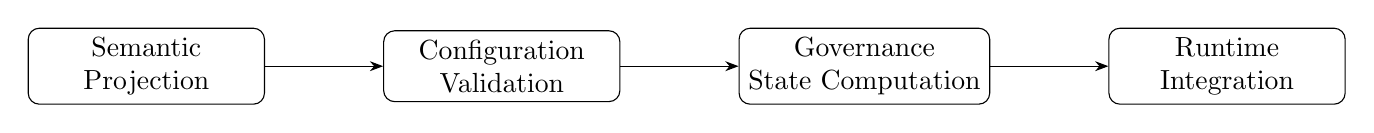
\begin{tikzpicture}[
node distance=1.5cm,
every node/.style={
draw,
rounded corners,
align=center,
minimum width=3cm,
minimum height=0.8cm
},
>=Stealth
]

\node (projection) {Semantic\\Projection};
\node (validation) [right=of projection] {Configuration\\Validation};
\node (states) [right=of validation] {Governance\\State Computation};
\node (runtime) [right=of states] {Runtime\\Integration};

\draw[->] (projection) -- (validation);
\draw[->] (validation) -- (states);
\draw[->] (states) -- (runtime);

\end{tikzpicture}

\caption{Governance processing pipeline implemented by the reference operationalization.}
\label{fig:governance_processing_pipeline}
\end{figure}

\subsubsection{Processing Stage 1: Semantic Projection}

The first processing stage transforms framework-specific configuration artifacts into ACM concepts according to the semantic projection rules introduced in Section~\ref{sec:semantic_projection}. The objective is to preserve governance-relevant semantics rather than reproduce the native internal representation of the originating framework.

\begin{algorithm}[ht]
\caption{Semantic Projection}
\KwIn{Native framework configuration $F$}
\KwOut{Projected ACM objects}

Extract native artifacts\;

Apply framework-specific projection rules\;

Create projected ACM objects\;

Preserve provenance metadata\;

\Return projected configuration\;

\end{algorithm}

The resulting representation remains independent of governance processing and serves as the input to the normalization and validation stages.

\subsubsection{Processing Stage 2: Configuration Validation}

Configuration validation verifies that the projected ACM representation satisfies the structural constraints required by the reference model before governance states are computed.

Validation is intentionally deterministic and independent of runtime execution. It verifies object identities, reference consistency, relationship integrity, digest computation, and structural constraints while preserving the immutability of validated revisions.

\begin{algorithm}[ht]
\caption{Configuration Validation}
\KwIn{Normalized ACM configuration}
\KwOut{Validated configuration}

Resolve references\;

Verify structural constraints\;

Compute canonical digests\;

Detect structural inconsistencies\;

Produce validation report\;

\Return validated configuration\;

\end{algorithm}

Only validated ACM representations are processed by the governance engine.

\subsubsection{Processing Stage 3: Governance State Computation}

Once the configuration has been validated, governance states are computed according to the formal semantics introduced in Section~\ref{sec:governance_semantics}. This stage evaluates lifecycle status, impact propagation, eligibility, and assurance until a deterministic fixed point is reached.

Unlike lifecycle states, which remain intrinsic properties of immutable revisions, computed governance states are derived from the dependency structure of the configuration graph and may therefore evolve whenever dependencies change.

\begin{algorithm}[ht]
\caption{Governance State Computation}
\KwIn{Validated ACM configuration}
\KwOut{Computed governance states}

Initialize computed states\;

Repeat

\Indp

Compute impact propagation\;

Update eligibility\;

Update assurance\;

\Indm

Until convergence\;

\Return governed configuration\;

\end{algorithm}

Because propagation is deterministic over a finite configuration graph, convergence always produces a unique governance state for a given configuration and governance policy.

\subsubsection{Processing Stage 4: Runtime Integration}

The final processing stage incorporates runtime observations into the governance model without modifying immutable configuration artifacts. Runtime signals are normalized into ACM runtime events and integrated into the Runtime Graph introduced in Section~\ref{sec:governance_semantics}.

This separation preserves the distinction between governed configurations and operational execution while enabling replay, auditing, and runtime traceability.

\begin{algorithm}[ht]
\caption{Runtime Integration}
\KwIn{Runtime events}
\KwOut{Updated Runtime Graph}

Normalize runtime events\;

Update runtime graph\;

Maintain provenance\;

Enable replay reconstruction\;

\Return runtime representation\;

\end{algorithm}

Since runtime integration operates exclusively on normalized events, the resulting Runtime Graph remains independent of the native event formats exposed by individual execution frameworks.

\subsection{Reference Implementation}
\label{sec:reference_implementation}

The ACM reference model is operationalized through an open-source Python reference implementation developed to validate the feasibility of the proposed concepts and governance semantics. The implementation is intentionally presented as a reference operationalization rather than as a production-ready governance platform. Its primary objective is to demonstrate that the reference model can be realized using deterministic processing stages while remaining independent of any particular execution framework.

The implementation follows the layered architecture introduced in Section~\ref{sec:operationalization}. Framework-specific adapters are responsible for semantic projection, whereas the governance kernel operates exclusively on normalized ACM representations. This architectural separation ensures that governance algorithms remain independent of framework-specific execution models and may therefore be reused by future adapters without modification.

The implementation organizes configuration artifacts as immutable Agentic Configuration Item (ACI) revisions represented through strongly typed data models. Canonical serialization and content-addressed digests provide stable identities for configuration revisions, enabling deterministic comparison, provenance tracking, baseline management, and reproducible replay of governed configurations.

Governance processing is implemented as a deterministic pipeline corresponding directly to the formal semantics introduced in Section~\ref{sec:governance_semantics}. Configuration validation, lifecycle management, governance state computation, and runtime integration operate on immutable configuration revisions without modifying the underlying configuration artifacts. Runtime observations are maintained separately within the Runtime Graph, preserving the conceptual distinction between governed configurations and operational execution.

The modular organization of the reference implementation also facilitates extensibility. Supporting an additional agentic framework only requires the implementation of a new semantic projection adapter capable of producing normalized ACM artifacts. Since all subsequent governance processing operates exclusively on the normalized representation, no modification of the governance kernel is required when integrating additional frameworks.

Finally, the reference implementation serves as the experimental artifact supporting the evaluation presented in Section~\ref{sec:evaluation}. All normative scenarios, automated validation procedures, and cross-framework projection experiments reported in this paper are executed using this implementation, providing empirical evidence that the ACM reference model can be operationalized consistently while preserving framework-independent governance semantics.

\begin{table}[ht]
\centering
\caption{Correspondence between ACM concepts and the reference implementation.}
\label{tab:implementation_mapping}
\begin{tabular}{ll}
\toprule
\textbf{ACM Concept} & \textbf{Reference Implementation} \\
\midrule
Reference Model & Strongly typed ACI data models \\
Semantic Projection & Framework adapters \\
Governance Processing & Deterministic governance kernel \\
Configuration Graphs & Canonical graph representations \\
Runtime Semantics & Runtime event normalization \\
Reference Operationalization & Python implementation \\
\bottomrule
\end{tabular}
\end{table}


\section{Evaluation}
\label{sec:evaluation}

The previous section demonstrated how the ACM reference model can be operationalized through a framework-independent governance architecture, semantic projection pipeline, and reference implementation. The remaining question is whether this operationalization effectively preserves the governance semantics defined by the reference model while supporting heterogeneous agentic frameworks in practice.

The objective of this evaluation is therefore not to benchmark execution performance or compare orchestration frameworks. Instead, it assesses the extent to which the ACM reference model provides a consistent and operational foundation for configuration governance across heterogeneous agentic systems. More specifically, the evaluation investigates whether configurations originating from different frameworks can be projected into a common representation while preserving governance-relevant semantics and enabling deterministic governance processing.

The evaluation is conducted using the Python reference implementation presented in Section~\ref{sec:operationalization}. Two representative agentic frameworks, LangGraph and CrewAI, are used as experimental case studies because they embody distinct orchestration paradigms while remaining sufficiently mature and widely adopted within the current agentic ecosystem. The experimental protocol combines semantic projection experiments, normative governance scenarios, automated validation procedures, and runtime integration experiments in order to assess the operational feasibility of the proposed reference model.

The remainder of this section is organized as follows. Section~7.1 introduces the research questions guiding the evaluation. Section~7.2 describes the experimental methodology. Section~7.3 presents the experimental results, while Section~7.4 discusses their implications with respect to the objectives of the ACM reference model.

\subsection{Evaluation Objectives}
\label{sec:evaluation_objectives}

The evaluation aims to determine whether the ACM reference model fulfills the objectives defined throughout this paper. Rather than evaluating implementation-specific characteristics, the experiments focus on validating the conceptual properties of the reference model, its governance semantics, and its ability to provide a common governance layer across heterogeneous agentic frameworks.

To structure the evaluation, four research questions are defined.

\begin{itemize}

\item \textbf{RQ1 -- Expressiveness.}
Can the ACM reference model represent heterogeneous agentic configurations originating from different orchestration frameworks using a common governance representation?

\item \textbf{RQ2 -- Governance Preservation.}
Does semantic projection preserve the governance-relevant semantics of native configurations, including configuration identity, provenance, dependency relationships, lifecycle information, and runtime traceability?

\item \textbf{RQ3 -- Operational Feasibility.}
Can the governance semantics introduced in this paper be operationalized through a deterministic processing pipeline supporting configuration validation, governance state computation, and runtime integration?

\item \textbf{RQ4 -- Framework Independence.}
Can identical governance mechanisms be applied to configurations originating from structurally different frameworks without modifying the governance kernel?

\end{itemize}

These research questions directly reflect the principal design objectives introduced in Sections~3--6. Consequently, the evaluation does not attempt to compare the execution capabilities of individual agentic frameworks. Instead, it investigates whether ACM succeeds in abstracting framework-specific configuration models into a unified governance representation while preserving the semantics required for configuration management.

The following sections describe the experimental methodology adopted to answer these research questions and present the empirical evidence collected using the reference implementation.

\begin{table}[ht]
\centering
\caption{Research questions and evaluation criteria.}
\label{tab:research_questions}
\begin{tabular}{p{1cm} p{4.6cm} p{5.8cm}}
\toprule
\textbf{RQ} & \textbf{Objective} & \textbf{Evaluation Evidence} \\
\midrule
RQ1 & Assess the expressiveness of the ACM representation & Cross-framework semantic projection \\
RQ2 & Assess governance semantics preservation & Projection outcome analysis and governance validation \\
RQ3 & Assess operational feasibility & Automated governance scenarios and deterministic processing \\
RQ4 & Assess framework independence & Cross-framework execution of identical governance mechanisms \\
\bottomrule
\end{tabular}
\end{table}
\subsection{Experimental Methodology}
\label{sec:experimental_methodology}

The experimental methodology was designed to evaluate the ACM reference model with respect to the research questions introduced in Section~\ref{sec:evaluation_objectives}. Rather than measuring execution performance, the experiments assess whether heterogeneous agentic configurations can be governed through a common configuration model while preserving the governance semantics defined throughout this paper.

All experiments were conducted using the Python reference implementation described in Section~\ref{sec:reference_implementation}. This implementation realizes the semantic projection pipeline, governance processing stages, and runtime integration mechanisms introduced in Section~\ref{sec:operationalization}. It serves exclusively as an experimental artifact supporting the evaluation of the reference model.

Two representative agentic frameworks were selected as experimental case studies:

\begin{itemize}
\item \textbf{LangGraph}, representing explicit graph-based orchestration;
\item \textbf{CrewAI}, representing declarative agent-task orchestration.
\end{itemize}

These frameworks were intentionally chosen because they rely on different orchestration abstractions while exposing sufficiently rich configuration models to evaluate the framework-independence of ACM.

The evaluation combines four complementary experimental activities:

\begin{enumerate}

\item semantic projection of native framework configurations into normalized ACM representations;

\item execution of normative governance scenarios covering lifecycle management, dependency propagation, assurance evaluation, and runtime semantics;

\item automated validation of governance invariants and deterministic processing through the reference implementation;

\item comparative analysis of governance behavior across both frameworks.

\end{enumerate}

This methodology provides complementary evidence regarding both the conceptual validity of the ACM reference model and its practical operationalization. While semantic projection evaluates the expressiveness of the reference model, the governance scenarios validate the formal semantics introduced in Section~\ref{sec:governance_semantics}. Automated validation ensures that governance processing remains deterministic and reproducible, whereas the comparative analysis assesses the framework independence of the proposed governance architecture.

\begin{table}[ht]
\centering
\caption{Experimental protocol used to evaluate the ACM reference model.}
\label{tab:experimental_protocol}

\begin{tabular}{p{3.8cm}p{3.8cm}p{4.4cm}}
\toprule
\textbf{Experimental Activity} &
\textbf{Objective} &
\textbf{Research Questions} \\
\midrule

Semantic Projection &
Evaluate representational expressiveness &
RQ1, RQ2 \\

Governance Scenarios &
Validate governance semantics &
RQ2, RQ3 \\

Automated Validation &
Verify deterministic governance processing &
RQ3 \\

Cross-framework Comparison &
Assess framework independence &
RQ1, RQ4 \\

\bottomrule
\end{tabular}

\end{table}

\begin{figure}[ht]
\centering

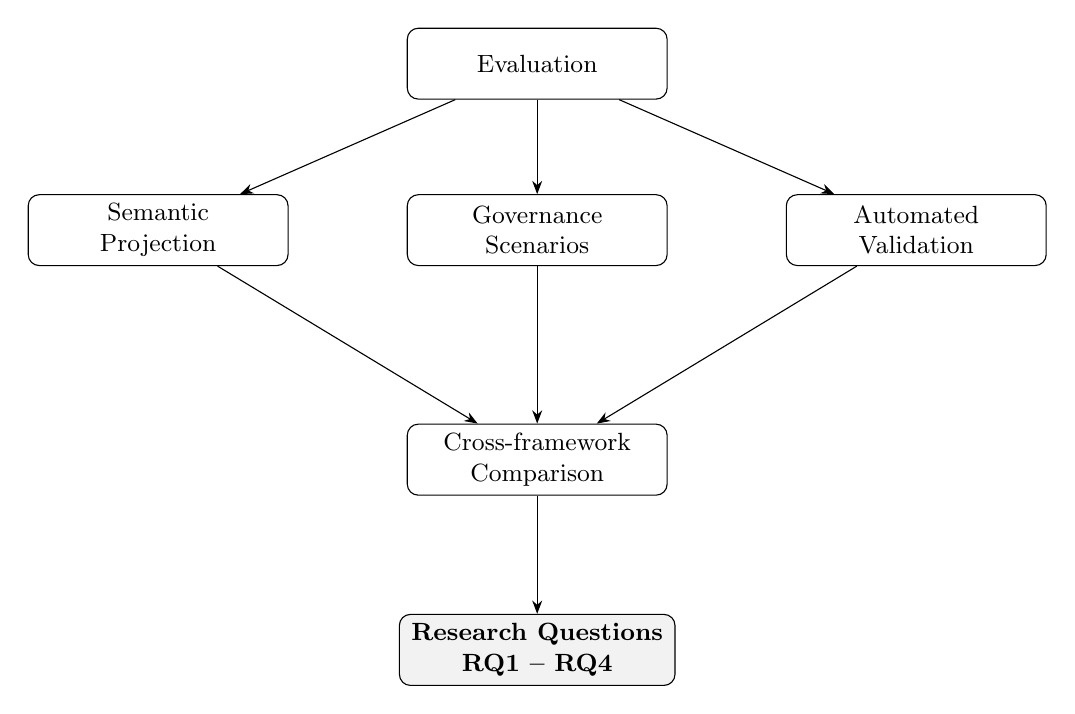
\begin{tikzpicture}[
node distance=1.2cm and 1.5cm,
>=Stealth,
process/.style={
draw,
rounded corners,
align=center,
minimum width=3.3cm,
minimum height=0.9cm,
font=\small
},
rq/.style={
draw,
rounded corners,
fill=gray!10,
align=center,
minimum width=3.5cm,
minimum height=0.9cm,
font=\small\bfseries
}
]

% Top
\node[process] (eval) {Evaluation};

% Middle row
\node[process, below left=of eval] (projection) {Semantic\\Projection};

\node[process, below=of eval] (scenarios) {Governance\\Scenarios};

\node[process, below right=of eval] (validation) {Automated\\Validation};

% Comparison
\node[process, below=2.0cm of scenarios] (comparison)
{Cross-framework\\Comparison};

% Bottom
\node[rq, below=1.5cm of comparison]
(rqs)
{Research Questions\\RQ1 -- RQ4};

% Connections
\draw[->] (eval) -- (projection);
\draw[->] (eval) -- (scenarios);
\draw[->] (eval) -- (validation);

\draw[->] (projection) -- (comparison);
\draw[->] (scenarios) -- (comparison);
\draw[->] (validation) -- (comparison);

\draw[->] (comparison) -- (rqs);

\end{tikzpicture}

\caption{Experimental methodology adopted to evaluate the ACM reference model. Complementary experimental activities collectively provide evidence for answering the research questions.}

\label{fig:evaluation_methodology}

\end{figure}

\subsection{Evaluation Results}
\label{sec:experimental_results}

This section presents the experimental evidence collected using the methodology described in Section~\ref{sec:experimental_methodology}. The objective is not to evaluate execution performance, but to assess whether the ACM reference model satisfies the research questions introduced in Section~\ref{sec:evaluation_objectives}. The reported results are derived from the latest validation and preservation reports generated by the reference implementation.

The evaluation addresses four complementary dimensions: (i) the representational expressiveness of ACM, (ii) the preservation of governance semantics during semantic projection, (iii) the deterministic operationalization of the governance model, and (iv) the framework-independent behavior of the governance kernel.

\subsubsection{Model Expressiveness}

The first objective of the evaluation is to determine whether heterogeneous agentic configurations can be represented using the common ACM metamodel.

The evaluated workflows extracted from LangGraph and CrewAI were successfully normalized into the ACM representation introduced in Section~\ref{sec:reference_model}. Despite relying on substantially different orchestration paradigms, both frameworks were represented through the same set of Agentic Configuration Items (ACIs), normalized relationships, immutable revisions, and governance metadata.

The evaluation therefore provides evidence that the ACM metamodel is sufficiently expressive to capture the principal governance concepts required by the evaluated agentic systems without introducing framework-specific abstractions into the governance layer.

\subsubsection{Governance Semantics Preservation}

A principal objective of semantic projection is the preservation of governance-relevant semantics rather than the exact reproduction of native framework implementations.

According to the preservation reports, both evaluated adapters preserve all structural elements within the normative ACM scope. Nodes, structural relationships, workflow branches, entry points, terminal nodes, prompt references, tool references, and canonical configuration digests are preserved for the evaluated workflows. Repeated projections produce identical canonical digests, demonstrating deterministic normalization.

The only remaining approximations concern execution semantics that are intentionally opaque to the native frameworks themselves. In particular, conditional routing logic implemented through arbitrary Python functions cannot be reconstructed statically and is therefore represented as an abstract routing structure. Likewise, CrewAI Flow state schemas currently remain outside the normative ACM scope and are consequently classified as unsupported rather than reconstructed.

Importantly, these limitations affect execution-specific implementation details rather than the governance semantics required by ACM. Configuration identity, provenance, dependency relationships, lifecycle information, runtime traceability, and configuration validation remain fully preserved throughout the projection process.

\begin{table}[ht]
\centering
\caption{Governance semantics preservation for the evaluated workflows.}
\label{tab:preservation_summary}

\begin{tabular}{lccc}
\toprule
\textbf{Governance Property} &
\textbf{Preserved} &
\textbf{Approximated} &
\textbf{Unsupported} \\
\midrule
Configuration identity & \checkmark & & \\
Revision provenance & \checkmark & & \\
Dependency graph & \checkmark & & \\
Prompt references & \checkmark & & \\
Tool references & \checkmark & & \\
Canonical digests & \checkmark & & \\
Conditional routing semantics & & \checkmark & \\
Framework-specific runtime state & & & \checkmark \\
\bottomrule
\end{tabular}

\end{table}

\subsubsection{Operational Results}

The operational behavior of the reference implementation was evaluated through automated validation, executable governance scenarios, and deterministic propagation experiments.

The validation report executes a total of 277 automated tests without failures or skipped tests. In addition, twenty-seven normative governance scenarios covering configuration integrity, propagation semantics, runtime replay, dynamic agents, permission management, portability, and robustness are executed through a common validation harness.

Deterministic propagation is further evaluated through eleven declarative propagation scenarios expressed independently from the Python implementation. These fixtures verify the convergence of the governance engine under representative dependency structures and provide additional confidence that governance semantics are determined by the specification rather than by implementation-specific behavior.

Collectively, these results demonstrate that the governance semantics defined in Section~\ref{sec:governance_semantics} can be operationalized through a deterministic processing pipeline while maintaining reproducible configuration identities, immutable revisions, deterministic propagation, and replayable runtime behavior.

\begin{table}[ht]
\centering
\caption{Summary of experimental results.}
\label{tab:experimental_results}

\begin{tabular}{lr}
\toprule
\textbf{Evaluation Metric} & \textbf{Result} \\
\midrule
Automated tests & 277 passed \\
Failed tests & 0 \\
Skipped tests & 0 \\
Normative scenarios & 27 \\
Propagation fixtures & 11 \\
Projection determinism & Confirmed \\
Canonical digest stability & Confirmed \\
Runtime replay & Successful \\
\bottomrule
\end{tabular}

\end{table}

\subsection{Discussion of Results}
\label{sec:discussion_results}

The experimental results provide empirical evidence supporting the principal objectives of the ACM reference model. Rather than evaluating execution performance, the experiments were designed to assess whether ACM provides a consistent governance abstraction capable of representing heterogeneous agentic systems while preserving the governance semantics introduced throughout this paper.

The discussion is therefore organized according to the four research questions introduced in Section~\ref{sec:evaluation_objectives}.

\subsubsection*{RQ1 -- Expressiveness}

The evaluation demonstrates that the ACM metamodel is sufficiently expressive to represent heterogeneous agentic configurations originating from structurally different orchestration frameworks. Both LangGraph and CrewAI configurations were successfully normalized into a common representation composed of immutable Agentic Configuration Items (ACIs), typed relationships, governance metadata, and runtime artifacts.

This result suggests that the abstraction level adopted by ACM captures governance-relevant concepts independently of the implementation paradigms used by individual frameworks. Rather than modeling framework-specific execution mechanisms, ACM focuses on the stable configuration concepts required for governance, traceability, and lifecycle management.

\subsubsection*{RQ2 -- Governance Preservation}

The preservation analysis indicates that semantic projection successfully maintains the governance semantics required by the reference model. Configuration identity, provenance, dependency relationships, lifecycle information, and canonical revisions remain preserved after normalization.

The few observed limitations primarily concern execution-specific constructs that are intentionally excluded from the normative ACM scope. For example, arbitrary routing functions implemented through general-purpose programming languages cannot be reconstructed statically without introducing framework-dependent interpretation. Likewise, framework-specific runtime state representations remain native execution concerns rather than governance artifacts.

These observations reinforce one of the central design principles of ACM: semantic projection aims to preserve governance semantics rather than reproduce every implementation detail of the originating framework.

\subsubsection*{RQ3 -- Operational Feasibility}

The automated validation procedures and normative governance scenarios demonstrate that the governance semantics introduced in this paper can be operationalized through a deterministic processing pipeline.

The successful execution of automated validation, deterministic propagation scenarios, immutable revision management, and runtime replay confirms that the proposed governance semantics are not merely conceptual definitions but can be implemented consistently through a practical software architecture.

Although the current implementation should be regarded as a reference operationalization rather than a production platform, the obtained results provide evidence that the reference model is technically realizable without introducing framework-specific governance mechanisms.

\subsubsection*{RQ4 -- Framework Independence}

Perhaps the most significant outcome of the evaluation is the observed independence between governance processing and framework-specific execution models.

Once native configurations have been normalized into ACM artifacts, all subsequent governance stages—including validation, lifecycle management, impact propagation, assurance evaluation, and runtime integration—operate without requiring knowledge of the originating framework. The framework adapters therefore constitute the only framework-dependent components of the architecture.

It should nevertheless be emphasized that the current evaluation remains limited to two representative frameworks. While the obtained results strongly support the feasibility of framework-independent governance, broader validation involving additional orchestration paradigms will be necessary to further strengthen the generalizability of the proposed reference model.

\subsubsection*{Overall Assessment}

Taken together, the experimental results support the central hypothesis of this work: governance can be decoupled from execution by introducing a normalized configuration layer preserving governance semantics independently of framework-specific implementations.

The evaluation therefore provides initial empirical evidence that the ACM reference model constitutes a practical and coherent foundation for Agentic Configuration Management. At the same time, the limited number of evaluated frameworks naturally constrains the scope of the conclusions. Extending the evaluation to additional orchestration ecosystems constitutes an important direction for future work, as discussed in Section~10.

\begin{table}[ht]

\centering

\caption{Summary of research question outcomes.}

\label{tab:rq_summary}

\begin{tabular}{p{1cm}p{2.7cm}p{5cm}p{2cm}}

\toprule

\textbf{RQ} &
\textbf{Objective} &
\textbf{Evidence} &
\textbf{Outcome}

\\

\midrule

RQ1 &
Expressiveness &
Successful cross-framework representation &
Supported

\\

RQ2 &
Governance preservation &
Semantic preservation analysis &
Supported

\\

RQ3 &
Operational feasibility &
Automated validation and deterministic processing &
Supported

\\

RQ4 &
Framework independence &
Identical governance processing across frameworks &
Supported within evaluated scope

\\

\bottomrule

\end{tabular}

\end{table}

\section{Discussion}
\label{sec:discussion}
\subsection{Positioning with Respect to Existing Agentic Frameworks}
\label{sec:positioning}

The rapid emergence of agentic frameworks has significantly simplified the development of LLM-based applications by providing increasingly sophisticated abstractions for workflow orchestration, agent coordination, tool integration, and execution management. Frameworks such as LangGraph and CrewAI exemplify this evolution by exposing distinct orchestration paradigms tailored to different classes of agentic systems.

The objective of ACM is fundamentally different. Rather than providing execution capabilities, ACM introduces a framework-independent governance layer dedicated to the management of agentic configurations throughout their lifecycle. Consequently, ACM should not be interpreted as an alternative orchestration framework, but as a complementary governance model capable of operating across heterogeneous execution environments.

This distinction is reflected in the responsibilities addressed by each approach. Agentic frameworks primarily define how agents execute, communicate, and coordinate during runtime. ACM, by contrast, governs what is being executed by providing immutable configuration revisions, provenance tracking, lifecycle management, dependency analysis, baseline management, assurance evaluation, and runtime traceability. Execution and governance therefore constitute complementary concerns operating at different abstraction levels.

The semantic projection mechanism introduced in Section~\ref{sec:semantic_projection} provides the interface between these two layers. By translating framework-specific configurations into normalized ACM artifacts, governance processing becomes independent of the originating execution framework while preserving the governance semantics required for configuration management. This separation allows identical governance mechanisms to be applied to configurations originating from heterogeneous orchestration paradigms without introducing framework-specific logic into the governance kernel.

More generally, the proposed architecture aligns with the long-established separation between execution infrastructures and configuration management observed in traditional software engineering. Source code management systems, build systems, deployment platforms, and runtime environments have historically evolved as complementary but distinct components of the software lifecycle. ACM extends this principle to agentic systems by introducing an explicit governance layer dedicated to the management of agentic configurations rather than their execution.

The experimental evaluation presented in Section~\ref{sec:evaluation} provides initial evidence supporting this positioning. The successful projection of representative LangGraph and CrewAI workflows into a common ACM representation demonstrates that governance can be decoupled from execution while preserving the semantics required for configuration management. Although the current evaluation remains limited to two representative frameworks, the obtained results suggest that this architectural separation provides a viable foundation for framework-independent governance of agentic systems.

\begin{figure}[t]
    \centering

    \begin{tikzpicture}[
        font=\scriptsize,
        node distance=4mm and 3mm,
        layer/.style={
            draw,
            rounded corners=1.5pt,
            minimum width=0.94\columnwidth,
            inner xsep=4pt,
            inner ysep=5pt,
            align=center,
            line width=0.6pt
        },
        component/.style={
            draw,
            rounded corners=1pt,
            minimum height=6mm,
            inner xsep=4pt,
            inner ysep=2pt,
            align=center,
            line width=0.45pt
        },
        projection/.style={
            draw,
            minimum width=0.58\columnwidth,
            minimum height=6mm,
            align=center,
            line width=0.6pt
        },
        arrow/.style={
            -{Latex[length=2mm,width=1.3mm]},
            line width=0.65pt
        }
    ]

    % ---------------------------------------------------------
    % Execution layer
    % ---------------------------------------------------------

    \node[layer] (execution) {
        \textbf{Agentic Execution Frameworks}\\[4pt]
        \begin{tikzpicture}[
            baseline,
            component/.style={
                draw,
                rounded corners=1pt,
                minimum width=21mm,
                minimum height=6mm,
                align=center,
                line width=0.45pt
            }
        ]
            \node[component] (langgraph) {LangGraph};
            \node[component, right=2mm of langgraph] (crewai) {CrewAI};
            \node[component, right=2mm of crewai] (others) {Other Frameworks};
        \end{tikzpicture}
    };

    % ---------------------------------------------------------
    % Semantic projection
    % ---------------------------------------------------------

    \node[projection, below=5mm of execution] (projection) {
        \textbf{Semantic Projection}\\
        Framework-specific adapter and normalization
    };

    \draw[arrow] (execution) -- (projection);

    % ---------------------------------------------------------
    % ACM governance layer
    % ---------------------------------------------------------

    \node[layer, below=5mm of projection] (acm) {
        \textbf{ACM Framework-Independent Governance Layer}\\[4pt]
        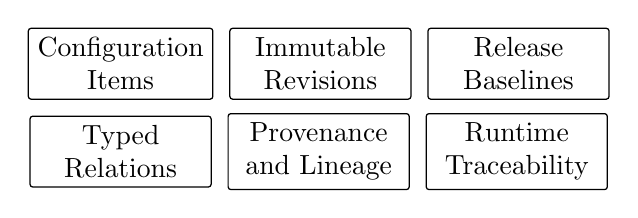
\begin{tikzpicture}[
            baseline,
            component/.style={
                draw,
                rounded corners=1pt,
                minimum width=23mm,
                minimum height=6mm,
                align=center,
                line width=0.45pt
            }
        ]
            \node[component] (aci) {Configuration\\Items};
            \node[component, right=2mm of aci] (revisions) {Immutable\\Revisions};
            \node[component, right=2mm of revisions] (baselines) {Release\\Baselines};

            \node[component, below=2mm of aci] (relations) {Typed\\Relations};
            \node[component, right=2mm of relations] (provenance) {Provenance\\and Lineage};
            \node[component, right=2mm of provenance] (runtime) {Runtime\\Traceability};
        \end{tikzpicture}
    };

    \draw[arrow] (projection) -- (acm);

    % ---------------------------------------------------------
    % Governance capabilities
    % ---------------------------------------------------------

    \node[layer, below=5mm of acm] (governance) {
        \textbf{Governance Capabilities}\\[4pt]
        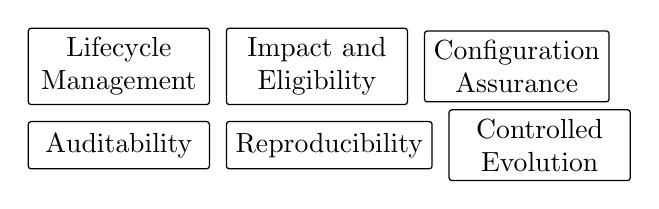
\begin{tikzpicture}[
            baseline,
            component/.style={
                draw,
                rounded corners=1pt,
                minimum width=23mm,
                minimum height=6mm,
                align=center,
                line width=0.45pt
            }
        ]
            \node[component] (lifecycle) {Lifecycle\\Management};
            \node[component, right=2mm of lifecycle] (impact) {Impact and\\Eligibility};
            \node[component, right=2mm of impact] (assurance) {Configuration\\Assurance};

            \node[component, below=2mm of lifecycle] (audit) {Auditability};
            \node[component, right=2mm of audit] (reproducibility) {Reproducibility};
            \node[component, right=2mm of reproducibility] (change) {Controlled\\Evolution};
        \end{tikzpicture}
    };

    \draw[arrow] (acm) -- (governance);

    \end{tikzpicture}

    \caption{Positioning of ACM with respect to agentic execution frameworks. Framework-specific configurations are semantically projected into a common governance representation, allowing lifecycle, assurance, traceability, and change-management mechanisms to operate independently of the originating framework.}
    \label{fig:acm_framework_positioning}
\end{figure}

\subsection{Contributions to Agentic Configuration Governance}
\label{sec:governance_contributions}

The contribution of ACM lies neither in introducing a new orchestration mechanism nor in extending the execution capabilities of existing agentic frameworks. Its primary contribution is to establish configuration governance as an explicit and framework-independent concern for agentic systems. From this perspective, ACM contributes at four complementary levels: representation, semantics, interoperability, and operational validation.

\subsubsection{A Framework-Independent Reference Model}

The first contribution is a reference model that represents an agentic system as a governed configuration rather than as a collection of framework-specific runtime objects. The model introduces explicit configuration items, immutable revisions, typed relationships, provenance information, and release baselines. These abstractions provide a common vocabulary for describing the constituent elements of an agentic system and the dependencies that determine its effective configuration.

This representation extends established configuration-management principles to artifacts that are specific to agentic systems. In particular, it treats agents, prompts, tools, policies, models, workflows, and dynamically instantiated components as governable objects whose identity and evolution can be tracked independently. The resulting configuration is therefore not reduced to source code, deployment metadata, or execution traces. It is represented as an explicit and auditable object in its own right.

A central consequence of this model is the ability to distinguish logical identity from immutable revision identity. Successive revisions of the same configuration item preserve a stable conceptual identity while remaining individually addressable through exact revision identifiers and content digests. This distinction supports reproducibility, comparison, controlled replacement, and historical reconstruction without conflating an evolving artifact with one of its concrete states.

\subsubsection{Formal Governance Semantics}

The second contribution is the formalization of governance semantics over the reference model. ACM does not merely describe which artifacts exist; it defines how their governance states evolve and how local changes affect dependent configurations.

The lifecycle model specifies admissible transitions for configuration revisions, baselines, and runtime instances. Quality, assurance, impact, and eligibility are maintained as distinct dimensions rather than being collapsed into a single status. This separation prevents ambiguous interpretations such as treating a lack of evidence as proof of poor quality or propagating the lifecycle state of a dependency directly to its parent.

The propagation semantics further define how dependency changes, invalidated evidence, deprecated components, and runtime deviations influence the governance status of composite configurations. These effects are restrictive rather than destructive: a problematic dependency may block the promotion of a composite configuration without rewriting the intrinsic quality or lifecycle state of that composite. The model thereby preserves the provenance of governance decisions while supporting deterministic and explainable state computation.

The assurance model complements these semantics by linking governance conclusions to explicit evidence. Validation and approval are attached to exact revisions and scopes, allowing the system to distinguish directly assessed artifacts from conclusions inherited through assurance-relevant dependencies. Governance states can therefore be interpreted together with the evidence and rules from which they were derived.

\subsubsection{Framework-Independent Semantic Projection}

The third contribution is the separation between framework-specific extraction and framework-independent governance processing. Native configurations are translated into ACM through semantic projection, while the governance kernel operates exclusively on normalized ACM artifacts.

This architecture allows heterogeneous orchestration paradigms to be governed through a common representation. A graph-oriented framework may expose nodes and edges directly, whereas a role- and task-oriented framework may require part of its topology to be reconstructed from assignments and dependencies. ACM does not require these native representations to be structurally identical. It requires the projection to preserve the information needed for configuration governance and to make approximated or unavailable information explicit.

Framework independence should therefore be understood as independence of the governance model and processing semantics from a specific execution framework. The adapters remain framework-specific because they interpret native concepts. Once projection is complete, however, lifecycle validation, baseline construction, dependency analysis, assurance computation, runtime integration, and impact propagation no longer depend on the source framework.

This separation provides a basis for interoperability without imposing a common execution model. Frameworks retain their native orchestration semantics, while ACM supplies a shared governance representation above them.

\subsubsection{Reference Operationalization and Evaluation}

The fourth contribution is the operationalization of the reference model through an executable implementation and its evaluation across two distinct agentic frameworks. The Python prototype demonstrates that the proposed abstractions and semantics can be implemented as deterministic processing mechanisms rather than remaining solely conceptual definitions.

The reference implementation operationalizes immutable revisions, canonical serialization, configuration validation, state propagation, baseline processing, runtime-event normalization, and replay. The LangGraph and CrewAI adapters instantiate the semantic-projection boundary for two frameworks with different native abstractions. Their use does not establish universal applicability, but provides initial evidence that the model can accommodate both explicit graph structures and role--task compositions.

The evaluation also contributes a structured validation methodology combining normative governance scenarios, automated tests, and semantic-preservation analysis. This methodology distinguishes successful representation from exact structural equivalence and records which governance-relevant properties are preserved, reconstructed, approximated, or unavailable. It therefore provides a more appropriate validation criterion for a reference model than conventional runtime-performance benchmarking.

Taken together, these four contributions establish ACM as a configuration-governance abstraction positioned between agentic execution environments and higher-level operational or organizational governance processes. The reference model defines what is governed, the formal semantics define how governance states are computed, semantic projection connects heterogeneous frameworks to the model, and the reference implementation demonstrates that these mechanisms can be operationalized consistently.

\subsection{Practical Implications}
\label{sec:practical_implications}

Beyond its conceptual contribution, ACM has practical implications for the engineering and governance of agentic systems. By introducing an explicit and framework-independent configuration representation, the proposed model enables governance activities that are difficult to perform when configuration information remains fragmented across framework-specific abstractions.

A first implication concerns reproducibility. In current agentic ecosystems, reproducing a previous execution often requires reconstructing configurations from multiple heterogeneous artifacts, including prompts, workflow definitions, deployment parameters, runtime traces, and external resources. ACM addresses this fragmentation by associating executions with immutable configuration revisions and controlled release baselines. A governed execution can therefore be traced back to the exact configuration from which it originated, supporting reproducible experiments, regression analyses, and long-term maintenance.

A second implication concerns auditability and traceability. Since governance decisions are explicitly linked to identified configuration revisions and supporting evidence, the provenance of a validation result or lifecycle transition becomes inspectable rather than implicit. This capability facilitates post-deployment analysis, compliance reporting, and forensic investigation by making configuration evolution transparent throughout the lifecycle of the system.

The explicit representation of dependencies also supports systematic change management. Instead of reasoning independently about prompts, agents, tools, or models, ACM represents these artifacts as interconnected configuration items whose relationships can be analyzed before modifications are promoted to a released baseline. Dependency-aware impact analysis provides early visibility into the potential consequences of configuration changes, reducing the likelihood of unintended regressions.

The proposed model also provides a common governance abstraction that may facilitate interoperability across heterogeneous execution environments. Organizations frequently combine multiple orchestration frameworks to address different operational requirements. By projecting these heterogeneous configurations into a shared governance representation, ACM enables governance policies to be expressed independently of the underlying execution technology while allowing each framework to preserve its native execution semantics.

Finally, ACM may contribute to the emerging AgentOps ecosystem by complementing existing observability and orchestration platforms with explicit configuration governance. Current operational platforms primarily focus on execution monitoring, tracing, evaluation, and operational metrics. ACM addresses a complementary concern by governing the configuration artifacts that determine how those executions are produced. Consequently, the model should be viewed as a governance layer that can coexist with, rather than replace, existing AgentOps and LLMOps infrastructures.

\subsection{Limitations of the Current Reference Model}
\label{sec:model_limitations}

Although the proposed reference model provides a comprehensive governance abstraction for the evaluated scenarios, several limitations remain inherent to its current scope.

First, ACM focuses on configuration governance rather than execution semantics. The model intentionally abstracts away framework-specific scheduling strategies, execution optimizations, concurrency mechanisms, and internal orchestration policies. While this separation is essential to preserve framework independence, it also implies that certain execution-specific behaviors cannot be represented explicitly within the governance model.

Second, semantic projection is inherently constrained by the information exposed by the originating framework. Native abstractions that are explicit in one framework may only be reconstructed indirectly in another, and some execution details may simply be unavailable through public interfaces. ACM therefore emphasizes governance semantics preservation rather than exact structural equivalence. The model explicitly acknowledges that certain information may be reconstructed, approximated, or unavailable after projection.

Third, the current model primarily governs explicitly identifiable configuration artifacts. Although runtime-created agents and dynamically instantiated components are incorporated through the runtime governance model, ACM does not attempt to infer the intent or internal decision-making process of autonomous agents. Instead, it governs the observable configuration artifacts and events that can be deterministically identified throughout execution.

Another limitation concerns the scope of governance itself. ACM deliberately concentrates on configuration management, provenance, lifecycle governance, assurance, and runtime traceability. Broader organizational concerns such as organizational risk management, regulatory compliance processes, human governance workflows, or enterprise policy management remain outside the scope of the reference model. These concerns can interact with ACM but are not represented directly within its metamodel.

Finally, the current reference model intentionally favors determinism, explainability, and implementation simplicity over exhaustive expressiveness. Governance decisions are derived from explicit artifacts, typed relationships, deterministic propagation rules, and identifiable evidence. More sophisticated reasoning mechanisms, including probabilistic governance models, adaptive propagation policies, or autonomous governance decisions, were intentionally excluded from the current specification in order to preserve the transparency and reproducibility expected from a configuration governance model.

These limitations do not invalidate the proposed approach; rather, they define the current scope of the reference model and identify directions in which future extensions may broaden its applicability while preserving its fundamental design principles.

\subsection{Section Summary}

This discussion has positioned ACM as a framework-independent reference model dedicated to the governance of agentic system configurations. Rather than introducing a new execution framework, ACM complements existing orchestration technologies by providing a common semantic foundation for representing, governing, and auditing heterogeneous agentic configurations throughout their lifecycle.

The proposed reference model combines a unified configuration representation with formal governance semantics and a framework-independent operationalization. The evaluation demonstrates that these concepts can be instantiated consistently across structurally different agentic frameworks while preserving the governance information required for lifecycle management, provenance, assurance, and reproducibility within the evaluated scope.

At the same time, the discussion has highlighted that ACM deliberately defines a minimal governance core rather than an exhaustive description of every abstraction introduced by current or future frameworks. Native concepts such as framework-specific orchestration constructs, execution optimizations, or emerging abstractions including reusable skills can be represented through semantic projection without requiring modifications to the underlying governance model, thereby preserving the framework independence that constitutes one of ACM's primary design principles.

The following section examines the principal threats to the validity of this study and discusses the methodological and experimental factors that should be considered when interpreting the reported results.

\section{Threats to Validity}
\label{sec:threats_validity}

The preceding sections presented the ACM reference model, its formal governance semantics, its operationalization through a reference implementation, and an experimental evaluation conducted across two heterogeneous agentic frameworks. Together, these elements provide evidence that the proposed model is internally consistent, operationally realizable, and capable of preserving governance semantics within the evaluated scope.

As with any reference model, however, these results must be interpreted within the boundaries of the assumptions, implementation choices, and experimental conditions that characterize the present study. The purpose of this section is therefore not to question the conceptual validity of ACM itself, but to identify the principal factors that may influence the interpretation, reproducibility, and generalization of the reported results.

Following established empirical research practice, we distinguish threats related to the scope of the reference model, the validation of its formal semantics, the internal validity of the experimental methodology, the external validity of the reported conclusions, and the reproducibility of the evaluation artifacts. These limitations define the current scope of evidence supporting ACM and naturally motivate the research directions discussed in the following section.

\subsection{Validity of the Reference Model}
\label{sec:validity_reference_model}

The primary objective of this study is to evaluate whether ACM provides a sufficiently expressive and framework-independent reference model for representing and governing heterogeneous agentic system configurations. Consequently, the reported results should be interpreted as evidence supporting the proposed reference model within the scope of the evaluated frameworks rather than as a demonstration of universal applicability.

The evaluation intentionally considers two agentic frameworks exhibiting substantially different orchestration paradigms. LangGraph exposes an explicit graph-based execution model in which structural dependencies are directly represented, whereas CrewAI adopts a higher-level organization centered on agents, roles, tasks, and crews. Successfully projecting these heterogeneous representations into a common ACM configuration model provides initial evidence that the proposed abstractions are not tied to a single execution paradigm. Nevertheless, the evaluation remains limited to these two representative frameworks.

Other categories of agentic systems, including architectures relying on dynamic handoffs, highly decentralized coordination mechanisms, large-scale enterprise orchestration platforms, or future framework abstractions, have not yet been experimentally evaluated. Although the semantic projection architecture was explicitly designed to accommodate heterogeneous native representations, additional adapters and experimental studies are required before broader claims regarding framework independence can be established empirically.

Accordingly, the conclusions drawn from this study should be understood as demonstrating \emph{framework portability} across two structurally distinct orchestration paradigms rather than complete framework independence. The latter remains a design objective of the reference model whose broader empirical validation constitutes an important direction for future work.

\begin{table}[ht]
\centering
\caption{Scope of the Reference Model Validation}
\label{tab:validation_scope}
\begin{tabular}{p{5.1cm}cc}
\toprule
\textbf{Validation Aspect} & \textbf{Evaluated} & \textbf{Future Validation} \\
\midrule
Graph-based orchestration & \checkmark & \\
Role/task-based orchestration & \checkmark & \\
Framework-independent governance kernel & \checkmark & \\
Dynamic handoff architectures & & \checkmark \\
Enterprise-scale orchestration platforms & & \checkmark \\
Emerging agentic abstractions (e.g., skills) & & \checkmark \\
Additional execution frameworks & & \checkmark \\
\bottomrule
\end{tabular}
\end{table}

\subsection{Validity of the Formal Semantics}
\label{sec:validity_formal_semantics}

The governance semantics introduced in this work define the formal behavior of the ACM reference model through explicit lifecycle state machines, deterministic state propagation, assurance composition, and runtime governance rules. Unlike purely conceptual reference models, these semantics are operationalized by a reference implementation that executes the corresponding state computations, validation procedures, and propagation algorithms. Consequently, the reported experimental results validate not only the structural expressiveness of the reference model but also the practical executability of its governance semantics.

Nevertheless, the present study should not be interpreted as providing a formal proof of correctness of the proposed semantics. The mathematical definitions establish the intended behavior of the governance model, while the reference implementation demonstrates that these semantics can be operationalized consistently for the evaluated scenarios. This constitutes constructive evidence of correctness through implementation and experimentation rather than a formal verification of the underlying mathematical system.

Several theoretical properties therefore remain outside the scope of the current work. In particular, the study does not formally prove properties such as termination of the fixed-point propagation process, confluence under alternative evaluation orders, completeness of semantic reconstruction across arbitrary frameworks, or the minimality of the computed governance states. Although the deterministic implementation and the successful execution of the validation scenarios provide empirical confidence that these properties hold within the evaluated scope, they have not yet been established through formal verification techniques.

Accordingly, the formal semantics should be regarded as an executable semantic specification supported by experimental evidence rather than as a mathematically verified formal system. Extending ACM with machine-checked proofs or theorem-based verification constitutes an important direction for future research and would further strengthen the theoretical foundations of the proposed governance model.

\subsection{Generalizability}
\label{sec:generalizability}

The evaluation reported in this study provides initial evidence that the ACM reference model can represent and govern heterogeneous agentic systems originating from multiple orchestration paradigms. Nevertheless, the scope of the experimental validation remains intentionally limited and should not be interpreted as demonstrating universal applicability across the rapidly evolving ecosystem of agentic frameworks.

The experimental study covers two representative but structurally distinct orchestration paradigms. LangGraph represents explicit graph-based orchestration, where execution structure and dependencies are directly modeled, whereas CrewAI represents a higher-level role- and task-oriented orchestration model requiring semantic reconstruction during projection. The successful projection of both frameworks supports the claim that ACM can normalize heterogeneous configuration representations while preserving the governance information required by the reference model.

\begin{table}[t]
\caption{Scope of the Experimental Validation}
\label{tab:validation_scope}
\centering
\begin{tabular}{p{4.0cm}cc}
\toprule
\textbf{Agentic System Category} & \textbf{Evaluated} & \textbf{Future Work} \\
\midrule
Graph-based orchestration (LangGraph) & \checkmark & \\
Role/task-based orchestration (CrewAI) & \checkmark & \\
Dynamic handoff architectures & & \checkmark \\
Hierarchical multi-agent delegation & & \checkmark \\
Swarm-based coordination & & \checkmark \\
Pipeline-oriented orchestration & & \checkmark \\
Large-scale enterprise deployments & & \checkmark \\
Cross-organizational governance & & \checkmark \\
\bottomrule
\end{tabular}
\end{table}

However, the evaluation does not yet include several important categories of agentic systems. Frameworks relying on dynamic handoffs, hierarchical delegation, decentralized swarms, large-scale distributed execution, or pipeline-oriented component orchestration may expose governance abstractions that are not currently represented in the evaluation corpus. Although the ACM metamodel was intentionally designed to remain independent of framework-specific abstractions, additional projection rules or extensions may prove necessary when addressing such architectures.

Similarly, the current experiments were conducted on normative governance scenarios and a reference implementation intended to validate the expressiveness and operational feasibility of the proposed model. They do not constitute an evaluation of industrial deployments involving thousands of configuration items, heterogeneous execution infrastructures, long-running production systems, or continuously evolving organizational governance processes.

Consequently, the conclusions of this study should be interpreted as evidence that ACM provides a viable framework-independent governance model for the classes of agentic systems evaluated, rather than as proof of universal applicability to every existing or future orchestration framework. Extending the empirical validation to additional ecosystems and deployment contexts constitutes an important direction for future work.

\subsection{Reproducibility and Replicability}
\label{sec:reproducibility}

Reproducibility constitutes a central objective of the ACM reference model and of the experimental methodology adopted in this work. Unlike traditional benchmarking studies focused on the probabilistic outputs of large language models, the present evaluation targets the deterministic governance layer that surrounds agentic systems. Consequently, the objective is not to reproduce identical LLM responses, but to reproduce identical governance states from equivalent configuration baselines and runtime evidence.

To support reproducibility, the reference implementation provides a complete governance pipeline composed of immutable configuration revisions, canonical serialization, deterministic state computation, replayable runtime events, and an automated validation suite. Together, these artifacts ensure that identical governed configurations produce identical governance outcomes independently of the underlying execution framework, provided that equivalent runtime evidence is supplied.

Similarly, the experimental protocol was designed to facilitate replicability by independent researchers. The reference implementation, the normative governance scenarios, the automated test suite, and the semantic projection adapters constitute explicit experimental artifacts that can be executed and inspected independently. This separation between the conceptual model, its operationalization, and the evaluation protocol reduces the dependence of the reported results on a specific implementation or execution environment.

\begin{figure}[t]
    \centering
    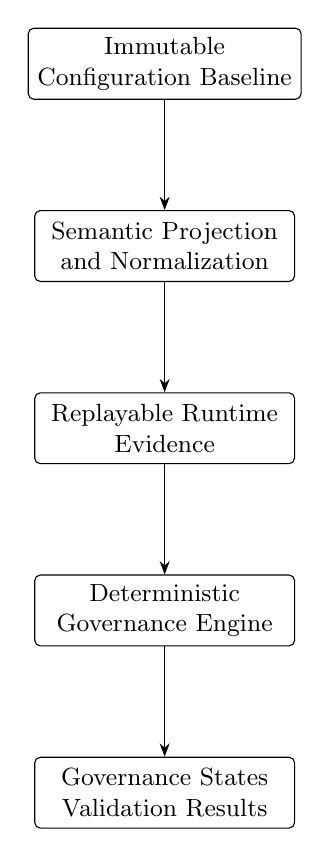
\begin{tikzpicture}[
    node distance=1.4cm,
    >=Stealth,
    box/.style={
        draw,
        rounded corners=2pt,
        align=center,
        minimum width=3.3cm,
        minimum height=0.9cm,
        font=\small
    }
]

\node[box] (baseline) {Immutable\\Configuration Baseline};

\node[box, below=of baseline] (projection) {Semantic Projection\\and Normalization};

\node[box, below=of projection] (runtime) {Replayable Runtime\\Evidence};

\node[box, below=of runtime] (engine) {Deterministic\\Governance Engine};

\node[box, below=of engine] (results) {Governance States\\Validation Results};

\draw[->] (baseline) -- (projection);
\draw[->] (projection) -- (runtime);
\draw[->] (runtime) -- (engine);
\draw[->] (engine) -- (results);

\end{tikzpicture}
    \caption{Deterministic governance pipeline supporting reproducibility and replicability. Immutable configuration baselines, semantic projection, replayable runtime evidence, and deterministic governance computation together enable independent reproduction of governance results without requiring deterministic LLM outputs.}
    \label{fig:reproducibility_pipeline}
\end{figure}

Nevertheless, complete reproducibility remains conditioned by the availability of semantically equivalent framework adapters and by the preservation of governance-relevant information during semantic projection. Furthermore, ACM intentionally abstracts from the probabilistic behavior of language models. Consequently, identical governance states do not imply identical generated outputs, but rather identical governed configurations, provenance information, lifecycle states, and governance decisions.

Overall, the reproducibility claims of this study concern the deterministic governance semantics defined by ACM and the associated evaluation methodology, rather than the stochastic behavior of the underlying AI models. This distinction is essential for interpreting the reported results and for comparing ACM with existing AgentOps and LLMOps evaluation approaches.

\subsection{Mitigation Strategies}
\label{sec:mitigation_strategies}

Although the preceding subsections identify several limitations affecting the present study, a number of methodological choices were deliberately adopted to reduce their impact on the reported results. Rather than attempting to maximize the breadth of the evaluation, the experimental methodology emphasizes internal consistency, deterministic governance semantics, and explicit separation between conceptual modeling, operationalization, and experimental validation.

First, the reference model was intentionally designed independently of any particular execution framework. The semantic projection architecture isolates framework-specific extraction mechanisms from the governance kernel, allowing the latter to remain unchanged across heterogeneous orchestration paradigms. This separation reduces implementation bias and facilitates the extension of the evaluation to additional frameworks without modifying the underlying governance semantics.

Second, the evaluation relies on normative governance scenarios rather than application-specific benchmarks. Each scenario targets a well-defined property of the reference model, such as lifecycle management, dependency propagation, assurance computation, baseline validation, or runtime governance. This scenario-driven methodology improves the traceability between the formal specification, the reference implementation, and the experimental evidence.

Third, reproducibility is reinforced through deterministic governance computation, immutable configuration revisions, canonical serialization, replayable runtime evidence, and automated validation procedures. These mechanisms ensure that governance outcomes depend exclusively on governed configurations and observed runtime events rather than on the stochastic behavior of the underlying language models.

Finally, the paper deliberately distinguishes between the conceptual reference model, its formal governance semantics, the reference implementation, and the experimental evaluation. This separation avoids conflating theoretical contributions with implementation artifacts and allows future implementations to validate the same governance semantics independently of the current prototype.

Table~\ref{tab:mitigation_strategies} summarizes the principal threats identified in this section together with the corresponding mitigation strategies adopted throughout the study.

\begin{table}[t]
\caption{Summary of Threats and Mitigation Strategies}
\label{tab:mitigation_strategies}
\centering
\begin{tabular}{p{4.2cm}p{3.9cm}}
\toprule
\textbf{Threat} & \textbf{Mitigation Strategy} \\
\midrule
Limited framework coverage &
Evaluation across heterogeneous orchestration paradigms; framework-independent governance kernel. \\

Incomplete formal verification &
Executable formal semantics supported by deterministic implementation and normative validation scenarios. \\

Limited empirical generalization &
Conservative interpretation of results; explicit delimitation of the evaluation scope. \\

Implementation-dependent bias &
Separation between semantic projection, governance kernel, and framework adapters. \\

Experimental reproducibility &
Immutable revisions, replayable runtime events, canonical serialization, and automated validation suite. \\

Framework evolution &
Projection architecture designed to accommodate additional adapters without modifying the reference model. \\
\bottomrule
\end{tabular}
\end{table}

\subsection{Section Summary}
\label{sec:threats_summary}

The objective of this section has been to delimit the scope within which the conclusions of the present study should be interpreted. The identified threats do not challenge the internal consistency of the ACM reference model nor the coherence of its governance semantics. Instead, they primarily concern the breadth of the experimental validation, the current level of formal verification, and the extent to which the reported results can be generalized across the rapidly evolving landscape of agentic systems.

The experimental methodology intentionally favors methodological rigor over exhaustive coverage by combining a framework-independent reference model, executable governance semantics, deterministic validation procedures, and reproducible experimental artifacts. Within this scope, the reported results provide credible evidence supporting the feasibility and expressiveness of the proposed governance model while avoiding claims that extend beyond the evaluated configurations.

These limitations naturally define the next stage of the research agenda. In particular, extending the empirical validation to additional orchestration paradigms, strengthening the formal verification of the governance semantics, and broadening the ecosystem supported by semantic projection represent logical continuations of the present work. These directions are discussed in the following section.

\section{Future Work}
\label{sec:future_work}

The ACM reference model introduced in this paper constitutes an initial step toward a framework-independent approach to the governance of agentic systems. The proposed metamodel, governance semantics, reference implementation, and experimental evaluation collectively demonstrate the feasibility of this approach within the scope considered in the present study. At the same time, the limitations identified in the previous section highlight several opportunities for extending both the theoretical foundations and the practical applicability of ACM.

Future research therefore naturally follows three complementary directions. The first concerns the evolution of the reference model itself to accommodate emerging abstractions while preserving its governance principles. The second focuses on strengthening the empirical and theoretical validation of the proposed semantics through broader experimental studies and formal verification. Finally, the long-term perspective is to position ACM as a common governance layer capable of interoperating with the rapidly expanding ecosystem of agentic development, deployment, and observability platforms.

\subsection{Extension of the Reference Model}
\label{sec:future_reference_model}

The reference model presented in this paper intentionally focuses on the minimal set of governance concepts required to represent heterogeneous agentic systems independently of their execution framework. This design choice favors conceptual stability and limits the number of core abstractions to those introducing distinct governance semantics. Nevertheless, the rapid evolution of agentic ecosystems will inevitably lead to the emergence of new configuration artifacts, interaction patterns, and execution abstractions that may require additional modeling capabilities.

A primary direction for future research is therefore the controlled evolution of the ACM metamodel while preserving its foundational design principles. Rather than continuously introducing framework-specific concepts into the core model, future extensions should remain guided by semantic necessity: a new abstraction should only become part of the reference model if it introduces governance properties that cannot be represented through the existing concepts and relationships. This principle preserves the framework independence of ACM while avoiding unnecessary growth of the metamodel.

An important example concerns reusable composite capabilities that are increasingly appearing under different names across modern agentic platforms, such as skills, reusable workflows, capability modules, or packaged execution components. Although these constructs differ in their implementation details, they frequently encapsulate existing governed artifacts—including prompts, tools, models, policies, workflows, and external resources—rather than introducing fundamentally new governance semantics. Consequently, many of these emerging abstractions can already be represented through semantic projection as governed composite configuration items without requiring modifications to the ACM core.

Future extensions may also address governance capabilities that extend beyond the scope of the current reference model. Examples include distributed governance across multiple organizations, federated configuration repositories, cross-system dependency management, richer policy composition mechanisms, and governance of long-lived autonomous ecosystems whose configuration evolves continuously over time. These extensions would broaden the applicability of ACM while preserving the separation between configuration governance and execution that constitutes one of its central architectural principles.

Ultimately, the long-term evolution of ACM should prioritize conceptual stability over feature accumulation. As with mature reference models in software engineering, the objective is not to mirror every innovation introduced by individual frameworks, but rather to identify the stable governance abstractions that remain applicable despite the continuous evolution of execution technologies. This philosophy enables the reference model to evolve incrementally while maintaining interoperability, explainability, and long-term sustainability.

\subsection{Broader Framework Validation}
\label{sec:future_framework_validation}

The empirical evaluation presented in this paper intentionally focuses on two representative orchestration paradigms in order to demonstrate the feasibility of framework-independent configuration governance. Although the successful semantic projection of LangGraph and CrewAI provides encouraging evidence supporting the proposed reference model, broader validation across the rapidly evolving landscape of agentic systems remains an essential research direction.

Future work should therefore extend the experimental corpus to additional execution frameworks exhibiting different orchestration principles and configuration abstractions. In particular, frameworks supporting dynamic handoffs, hierarchical delegation, event-driven coordination, decentralized multi-agent collaboration, or long-running autonomous workflows would provide valuable opportunities to evaluate the expressiveness of the ACM metamodel under substantially different execution models.

Beyond execution frameworks themselves, validation could also incorporate complementary components of the emerging AgentOps and LLMOps ecosystem. Provenance platforms, observability infrastructures, evaluation frameworks, and deployment management systems increasingly expose governance-relevant metadata that could naturally participate in semantic projection. Studying the integration of ACM with such platforms would provide additional evidence regarding the ability of the reference model to serve as a common governance layer across heterogeneous operational environments.

Another important direction concerns empirical validation at industrial scale. The current experiments intentionally emphasize semantic correctness rather than operational scalability. Future studies should therefore evaluate ACM on large agentic systems involving hundreds or thousands of governed configuration items, long-lived execution histories, continuously evolving baselines, and collaborative governance processes distributed across multiple development teams. Such evaluations would provide quantitative evidence regarding scalability, governance overhead, and operational usability in realistic production environments.

Ultimately, extending the experimental validation is not intended merely to increase the number of supported frameworks. Rather, it aims to progressively strengthen the empirical evidence supporting the central hypothesis of this work: that governance semantics can remain stable despite the continuous evolution of agentic execution technologies.

\subsection{Formal Verification of Governance Semantics}
\label{sec:future_formal_verification}

The governance semantics introduced in this paper are defined through a formal operational specification and validated through deterministic execution of the reference implementation. While this approach demonstrates the practical executability of the proposed semantics, it does not constitute a formal mathematical proof of their correctness. Establishing such guarantees represents an important direction for future research.

One immediate objective concerns the verification of the fixed-point propagation algorithm underlying governance state computation. Formal proofs could establish properties such as termination, determinism, convergence toward a unique governance state, and independence from evaluation order. Demonstrating these properties would strengthen confidence that governance decisions remain stable regardless of implementation details or execution strategies.

A second research direction involves the formal analysis of the lifecycle semantics themselves. The lifecycle state machines, dependency propagation rules, assurance composition mechanisms, and runtime governance semantics could be expressed within a formal verification framework in order to prove invariants such as transition consistency, absence of contradictory governance states, preservation of dependency constraints, and correctness of state propagation under arbitrary configuration topologies.

Beyond individual algorithms, future work may investigate the formal specification of the ACM reference model as a complete governance system. Model-checking techniques, temporal logic, theorem proving, or specification languages dedicated to distributed systems could be employed to verify global properties of the governance semantics and to detect inconsistencies automatically during the evolution of the reference model. Such approaches would complement the current implementation-based validation with machine-verifiable correctness guarantees.

Finally, formal verification would facilitate the development of independent ACM implementations. By providing mathematically specified governance semantics rather than relying solely on behavioral equivalence with the reference implementation, future implementations could demonstrate conformance through proof of semantic equivalence instead of implementation similarity. This evolution would represent an important step toward establishing ACM as a stable and implementation-independent governance specification.

\subsection{Toward an Agentic Configuration Ecosystem}
\label{sec:future_ecosystem}

The rapid maturation of agentic software engineering has led to the emergence of a rich ecosystem of complementary technologies dedicated to development, deployment, observability, evaluation, provenance, and operational governance. Rather than replacing these existing tools, ACM is intended to provide a framework-independent governance layer capable of connecting heterogeneous components through a common semantic representation of governed configuration artifacts.

A promising direction for future research therefore consists in studying the integration of ACM with broader AgentOps and LLMOps ecosystems. Modern observability platforms increasingly collect execution traces, evaluation results, model usage metrics, cost information, and provenance metadata that constitute valuable inputs for governance processes. Conversely, governance decisions produced by ACM could enrich these platforms with lifecycle status, assurance levels, configuration lineage, dependency analysis, and compliance information, providing a higher semantic level for operational monitoring.

Another important perspective concerns the integration of ACM with software engineering infrastructures. Continuous integration and deployment pipelines, software configuration management systems, artifact repositories, and supply-chain security mechanisms already manage the lifecycle of conventional software assets. Extending these infrastructures to incorporate governed agentic configuration items would enable unified governance across both traditional software components and AI-native artifacts while preserving traceability throughout the complete development lifecycle.

Beyond tooling integration, future work may explore the definition of interoperable governance services exposing standardized interfaces for semantic projection, configuration validation, governance state computation, and provenance exchange. Such services would facilitate the development of heterogeneous toolchains in which execution frameworks, observability platforms, deployment systems, and governance engines cooperate while remaining independently evolvable.

Ultimately, the long-term objective is to establish ACM not as another execution platform, but as a common semantic governance layer capable of interconnecting the diverse technologies that increasingly compose modern agentic software ecosystems.

\subsection{Standardization Perspectives}
\label{sec:future_standardization}

The absence of a common vocabulary and shared governance abstractions currently represents one of the principal obstacles to interoperability across agentic systems. While execution frameworks continue to evolve rapidly, equivalent concepts are frequently described using framework-specific terminology, making configuration exchange, governance portability, and comparative evaluation unnecessarily difficult.

The ACM reference model represents an initial step toward addressing this fragmentation by proposing a framework-independent conceptual vocabulary together with formally defined governance semantics. Although the present work does not aim to establish a standard, it provides a structured foundation upon which future community discussions regarding interoperable governance models may build.

Future research may therefore investigate the definition of standardized exchange formats for governed configuration items, semantic projection interfaces, governance evidence, provenance information, and lifecycle metadata. Such specifications would facilitate interoperability between heterogeneous execution frameworks while allowing governance information to remain portable independently of implementation technologies. Likewise, standardized conformance criteria could enable independent implementations to demonstrate semantic compatibility with the ACM reference model while preserving implementation freedom.

The maturation of ACM may also benefit from collaboration with broader software engineering and artificial intelligence communities working on software configuration management, software supply-chain security, provenance, and AI governance. Aligning ACM with existing standards whenever appropriate would facilitate its integration into established engineering practices while reducing duplication of concepts that are already well understood in adjacent disciplines.

Ultimately, the long-term ambition is not to standardize a particular implementation, but to encourage convergence toward a shared governance language for agentic systems. By separating governance semantics from execution technologies, ACM provides a stable conceptual foundation that could evolve collaboratively as the agentic ecosystem continues to mature. Such convergence would improve interoperability, reproducibility, auditability, and long-term sustainability across heterogeneous agentic platforms.

\section{Conclusion}
\label{sec:conclusion}

The rapid evolution of agentic software engineering has fundamentally transformed the role of configuration artifacts. Prompts, tools, execution graphs, policies, models, runtime state, and provenance have become first-class engineering assets whose governance can no longer rely solely on traditional software configuration management practices. At the same time, the increasing diversity of orchestration frameworks has introduced heterogeneous configuration abstractions, making governance difficult to reproduce, audit, and compare across platforms.

This paper introduced Agentic Configuration Management (ACM), a framework-independent reference model for the governance of agentic systems. Rather than proposing another execution framework, ACM separates governance semantics from execution technologies through a unified representation of governed configuration items, immutable revisions, semantic relationships, deterministic lifecycle management, assurance semantics, and runtime governance. This separation enables heterogeneous agentic systems to be represented within a common governance model while preserving the flexibility of existing orchestration frameworks.

Beyond the conceptual contribution, the paper demonstrated that the proposed semantics can be operationalized through a reference implementation and evaluated using representative orchestration paradigms. The experimental results show that heterogeneous agentic configurations can be semantically projected into a common governance representation while preserving the information required for deterministic governance decisions. Although the current evaluation remains intentionally limited in scope, it provides initial empirical evidence supporting the feasibility of framework-independent configuration governance for agentic systems.

More broadly, this work argues that governance should become an explicit architectural layer of agentic software engineering rather than an implementation-specific concern embedded within individual execution frameworks. By introducing a common vocabulary, formally defined governance semantics, and a framework-independent reference model, ACM establishes a foundation upon which future research can investigate interoperability, formal verification, scalable governance, and standardized configuration management practices for increasingly autonomous AI systems.

Ultimately, the contribution of ACM is not to prescribe how agentic systems should execute, but to provide a stable semantic foundation for governing how they are specified, versioned, validated, traced, and evolved. As agentic ecosystems continue to diversify, such a separation between execution and governance may become an essential prerequisite for building reproducible, auditable, interoperable, and trustworthy AI systems.

\section{Annexe}
\label{sec:annexe}
\begin{longtable}{p{0.9cm}p{2cm}p{6.2cm}p{2.3cm}p{1.6cm}}
\caption{Complete normative scenario catalogue.}
\label{tab:appendix_scenarios}\\

\toprule
ID &
Priority &
Normative objective &
Requirements &
Result \\
\midrule
\endfirsthead

\toprule
ID &
Priority &
Normative objective &
Requirements &
Result \\
\midrule
\endhead

S01 &
P0 &
Revision identity, immutable revisions and digest reproducibility &
I1--I4 &
Pass \\

S02 &
P0 &
Missing dependency detection and baseline consistency &
S02 &
Pass \\

S03 &
P0 &
Immutable revision history and append-only evolution &
S03 &
Pass \\

S04 &
P0 &
Baseline reproducibility from immutable revisions &
S04 &
Pass \\

S05 &
P0 &
Propagation of effective quality through dependencies &
S05 &
Pass \\

S06 &
P0 &
Eligibility propagation across dependent configuration items &
S06 &
Pass \\

S07 &
P0 &
Assurance coverage validation and dependency composition &
S07 &
Pass \\

S08 &
P1 &
Mixed quality propagation within heterogeneous dependency graphs &
S08 &
Pass \\

S09 &
P1 &
Propagation determinism under different traversal orders &
S09 &
Pass \\

S10 &
P1 &
Circular dependency detection and convergence guarantees &
S10 &
Pass \\

S11 &
P1 &
Fixed-point convergence of governance propagation &
S11 &
Pass \\

S12 &
P0 &
Runtime replay from immutable event log &
S12 &
Pass \\

S13 &
P0 &
Lifecycle transition validation during runtime replay &
S13 &
Pass \\

S14 &
P1 &
Declared runtime extension detection &
S14 &
Pass with deviation \\

S15 &
P1 &
Untraceable runtime instance detection &
S15 &
Pass with deviation \\

S16 &
P1 &
Configuration drift classification &
S16 &
Pass with deviation \\

S17 &
P0 &
Deterministic reconstruction of runtime state &
S17 &
Pass \\

S18 &
P1 &
Dynamic agent declaration and governance integration &
S18 &
Pass \\

S19 &
P1 &
Permission ceiling enforcement &
S19 &
Pass \\

S20 &
P1 &
Behaviour override validation &
S20 &
Pass \\

S21 &
P1 &
Promotion of dynamic agents into managed configuration &
S21 &
Pass \\

S22 &
P2 &
Projection consistency across supported frameworks &
S22 &
Pass \\

S23 &
P2 &
Framework-independent governance computation &
S23 &
Pass \\

S24 &
P2 &
Ordering invariance of normalized configuration &
S24 &
Pass \\

S25 &
P2 &
Robustness against incomplete framework metadata &
S25 &
Pass \\

S26 &
P2 &
Deterministic normalization of equivalent configurations &
S26 &
Pass \\

S27 &
P2 &
Local scalability on representative configuration graphs &
S27 &
Pass \\

\bottomrule
\end{longtable}

\begin{table}[t]
\centering
\caption{Provenance categories for normalized ACM information.}
\label{tab:information_provenance}
\begin{tabularx}{\linewidth}{lXX}
\toprule
Provenance category &
Definition &
Example \\
\midrule

Extracted &
Information obtained directly from an introspectable native framework object. &
LangGraph node or CrewAI agent \\

Declared by adapter &
Information explicitly supplied by the adapter when the native framework does not expose an equivalent static representation. &
Reconstructed CrewAI relationship \\

Derived &
Information deterministically computed from normalized ACM configuration or runtime data. &
Effective assurance or drift classification \\

Runtime-generated &
Information produced by an observed runtime event and appended to the event log. &
Agent creation or lifecycle transition \\

Unresolved &
Information whose value or semantics cannot be established from the available native objects or events. &
Opaque routing-function semantics \\

\bottomrule
\end{tabularx}
\end{table}
This provenance classification does not constitute a confidence or trust
assessment. It records how each item entered the ACM representation and enables
auditors to distinguish directly observed information from adapter declarations,
algorithmically derived values, runtime observations and unresolved semantics.
Assessing the reliability of these sources would require an additional
validation model and is outside the scope of the present evaluation.


\end{document}

